% ----------研究一
\chapter{研究一:AI生成个性化广告的初步实证}

为系统地检验AI在个性化广告创作中的能力,研究一通过四个实验逐步展开。实验1作为初步验证,采用GPT-3.5生成针对大五人格五个维度的高水平个性化广告,以评估AI生成广告的说服效果。实验2进一步考察AI在不同产品场景下的个性化广告生成能力,并采用GPT-4以探讨更强模型是否能提升个性化匹配效果。此外,该实验还检验了AI基于中性广告文本进行个性化改写的能力。实验3聚焦于不同人格水平(高 vs. 低)个体的匹配效果,探讨个性化广告是否能够有效吸引目标受众,并结合关键词分析考察不同群体在广告内容上的关注点。实验4则进一步分析AI在缺乏中性广告的情况下,能否直接基于产品描述生成个性化广告,并考察不同人格特质群体的广告偏好差异。通过这四个实验,研究一系统评估了AI在个性化广告创作中的适用性,并为后续研究提供了实证基础。

\section{实验1:AI生成个性化广告的初步检验}

\subsection{方法}
本实验旨在检验针对大五人格特质进行个性化广告设计的效果。在引导AI生成广告时,选用实验进行时表现最优的模型GPT-3.5。广告内容依据五种不同人格维度(外倾性、开放性、尽责性、宜人性、神经质)的高水平特质进行个性化设计,即分别为高外倾、高开放、高尽责、高宜人和高神经质的消费者进行个性化设计。GPT-3.5针对每种人格水平生成了3则广告,每位参与者在对应人格水平条件下随机观看其中一则广告。参与者依次观看针对大五人格五个维度设计的个性化广告,广告呈现顺序随机,且需对每则广告进行评价。

\textbf{(1)被试}

通过见数平台发布实验,200名参与者自愿参加这项研究。8名参与者由于注意检查测试未通过被剔除,剩余\textbf{192名}有效参与者(年龄范围= 18-58岁;\textit{M}=29.50岁;\textit{SD}=7.83;女性109名)。每名参与者完成实验后获得1元人民币作为报酬。注意力检测包含两部分,分别嵌入在因变量测量和人格问卷中,以明确指令题形式呈现(如“请选2”)。参与者需在两道注意力检测题中均作答正确,方可被纳入有效数据样本。

\textbf{(2)实验材料:广告设计}

实验共设计\textbf{5(广告人格:外倾性/开放性/尽责性/宜人性/神经质}的高水平设计共5个条件生成广告材料,采用GPT3.5生成。根据前人文献选择中性的产品手机,广告描述避免具体品牌名以排除品牌的影响。针对每个条件,GPT-3.5生成了5则广告文案,初始生成了25则广告材料。

在生成广告时,向GPT提供了结构化的提示语(prompt),包括目标消费者特点的描述、广告设计要求和基本特征描述。例如针对高外倾条件时的prompt如表\ref{tab:study1-exp-prompt}所示。提示语要求广告文案符合特定特质群体的需求,同时强调广告的说服力和针对性的语言表达。

\begin{table}[H]
    \caption{\label{tab:study1-exp-prompt} Prompt示例}
    {\tablesongti % 整个表格环境应用宋体六号字体
    \renewcommand{\arraystretch}{1} % 调整行距
    \begin{tabularx}{\linewidth}{lXc>{\centering\arraybackslash}X}
        \toprule
        \textbf{维度} & \textbf{Prompt} \\
        \midrule
        外倾性 & 请写五段有说服力的手机广告文案(每一段30字左右),需要满足下列要求: \newline
        1)广告呈现在社交媒体上(如小红书,微博等);\newline
        2)目标消费者特点是健谈的、精力充沛的、善于交际的、外向的、喜欢与他人互动的;\newline
        3)广告内容需要结合目标消费者特点和手机产品的特点;\newline
        4)广告目的是增加消费者购买的意愿,提高广告转化率。\newline
        \textbf{其他注意事项}:\newline
        避免出现“健谈”、“精力充沛”、“交际”、“外向”、“互动”等词语。\newline
        每一段可以变换一下句式。\newline
        不出现手机品牌。\newline
        注意是针对手机的广告(新增,担心文字多了GPT忘记是针对手机的广告)。 \\
        \bottomrule
    \end{tabularx}}
\end{table}

为验证生成的个性化广告是否能够有效传达针对目标消费者的特质,本研究在正式实验前通过见数平台发布了预实验,共有110名参与者自愿参加,完成实验后获得0.5元人民币作为报酬。预实验的筛选基于以下两个标准:1)目标消费者特质匹配性。参与者需对25则广告的目标消费者进行选择,任务为从5(人格特质)的高水平描述中选择最匹配的目标消费者。对于每则广告,若设计时对应的人格特质在选择中占比最高,则该广告被视为有效。例如,若广告是针对高外倾性设计的,而在选择结果中“高外倾性”选项占比最多,则表明该广告成功传达了高外倾性的特质;2)广告本身有效性。要求参与者对广告的理解程度与相关程度进行评分,采用1-5点量表,其中评分大于3分的广告被视为有效。经过预实验筛选,剩余15条(详见附录)。


\textbf{(3)问卷测量}
\label{study1-substudy1-measurement}

a. 大五人格量表。采用\citet{rammstedt2007measuring}编制的简版大五人格量表(Big Five Inventory,BFI-10,如表\ref{tab:BFI10-sample})测量参与者的人格特征。该量表共 10个项目,分属外倾性、宜人性、神经质、开放性、尽责性5个维度,每个维度有2道题目测量。参与者在1-5点李克特式量表上进行评分(选项“1”代表“非常不符合”,“5”代表“非常符合”)。

\begin{table}[H]
    \caption{\label{tab:BFI10-sample} BFI-10量表题目及计分方式}
    {\tablesongti % 整个表格环境应用宋体六号字体
    \renewcommand{\arraystretch}{1} % 调整行距
    \begin{tabularx}{\linewidth}{lXc>{\centering\arraybackslash}X}
        \toprule % 表格顶线
        序号 & 题目 & 人格 & 计分方式 \\ 
        \midrule % 表头下的中线
        1 & 总体而言是信任他人的 & 宜人性 & 正向 \\
        2 & 喜欢寻找别人的缺点   & 宜人性 & 反向 \\
        3 & 话不多              & 外倾性 & 反向 \\
        4 & 开朗,社交能力强     & 外倾性 & 正向 \\
        5 & 容易紧张或焦虑       & 神经质 & 正向 \\
        6 & 抗压能力强,容易放松 & 神经质 & 反向 \\
        7 & 想象力丰富           & 开放性 & 正向 \\
        8 & 对艺术不怎么感兴趣   & 开放性 & 反向 \\
        9 & 工作细致周到         & 尽责性 & 正向 \\
        10 & 懒惰               & 尽责性 & 反向 \\
        \bottomrule % 表格底线
    \end{tabularx}}
\end{table}

b. 说服效果。采用\citet{hirsh2012personalized}使用的五道题目测量广告的说服效果(表\ref{tab:persuasionSurvey}),包含参与者对广告的态度,以及对广告中产品的购买意愿。参与者需要在 5 点李克特式量表上对有关表述的同意程度进行评分(选项“1”代表“非常不同意”,“5”代表“非常统一”)。

\begin{table}[htbp]
    \caption{\label{tab:persuasionSurvey}广告说服效果量表}
    {\tablesongti % 整个表格环境应用宋体六号字体
    \renewcommand{\arraystretch}{1.5} % 调整行距
    \begin{tabularx}{\linewidth}{lXc>{\centering\arraybackslash}X}
        \toprule % 表头上方粗线
        序号 & 类别 & 题目 \\ 
        \midrule % 表头下方中线
        1 & 广告态度 & 这则广告让我对这个商品更感兴趣 \\ 
        2 & 广告态度 & 这则广告让我更想了解这个商品 \\ 
        3 & 广告态度 & 总的来说,我喜欢这则广告 \\ 
        4 & 购买意愿 & 我会考虑购买这个商品 \\ 
        5 & 购买意愿 & 如果我有需要,我会购买这个商品 \\ 
        \bottomrule % 表底粗线
    \end{tabularx}
    }
\end{table}

\subsection{实验流程}
本实验的流程分为两个部分。第一部分,参与者依次阅读每则广告,共5则广告,并对每组广告的相对说服效果进行评分。广告呈现顺序随机化,以控制顺序效应。第二部分,参与者需回答与人格测试相关的问卷题目,最后提供年龄、性别等人口统计学信息。

\subsection{结果}
为检验 AI(GPT-3.5)生成的个性化广告的有效性,本实验分别对每个特质的结果进行了回归分析。回归模型的自变量为参与者对应的人格特质得分(尽责性、开放性、外倾性、宜人性、神经质),因变量为个性化广告的说服效果。结果如表 \ref{tab:study1_traitResults} 所示。

回归分析结果表明,针对\textbf{宜人性} ($\beta = 0.2624, \textit{p} = 0.004$) 和 \textbf{外倾性} ($\beta = 0.1987, \textit{p} = 0.003$) 设计的个性化广告具有显著的说服效果,即个体的宜人性和外倾性水平越高,个性化广告的说服效果越好。此外,\textbf{开放性} 个体对个性化广告的接受度也呈现边缘显著的正向关系 ($\beta = 0.1394, \textit{p} = 0.060$),表明高开放性个体可能对AI生成的个性化广告表现出一定的偏好,但该效应仍需进一步检验。相比之下,\textbf{神经质} ($\beta = -0.1422, \textit{p} = 0.172$) 和 \textbf{尽责性} ($\beta = 0.0875, \textit{p} = 0.244$) 维度的个性化广告并未表现出显著的说服效果。整体而言,本研究的回归分析结果支持了 AI 生成的个性化广告在特定人格特质群体(如高宜人性和高外倾性个体)中的有效性,但其在特定人群中(如神经质,尽责性、开放性)的适用性和优化策略仍需进一步探讨。

\begin{table}[H]
    \centering
    \begin{threeparttable}
        \caption{\label{tab:study1_traitResults} 人格特质回归分析结果}
        {\tablesongti
        \renewcommand{\arraystretch}{1}
        \begin{tabular}{p{2cm} c c c c c c} 
            \toprule
            人格特质 & 系数 & 标准误差 & \textit{t} & \textit{P} $>|t|$ & [0.025 & 0.975] \\ 
            \midrule
            \textbf{宜人性} & \textbf{0.2624} & \textbf{0.091} & \textbf{2.876} & \textbf{0.004}\textsuperscript{**} & \textbf{0.082} & \textbf{0.442} \\
            \textbf{外倾性} & \textbf{0.1987} & \textbf{0.067} & \textbf{2.970} & \textbf{0.003}\textsuperscript{**} & \textbf{0.066} & \textbf{0.331} \\
            神经质 & -0.1422 & 0.104 & -1.370 & 0.172 & -0.348 & 0.063 \\
            尽责性 & 0.0875 & 0.075 & 1.167 & 0.244 & -0.061 & 0.236 \\
            \textbf{开放性} & \textbf{0.1394} & \textbf{0.074} & \textbf{1.894} & \textbf{0.060}\textsuperscript{\dag} & \textbf{-0.006} & \textbf{0.285} \\
            \bottomrule
        \end{tabular}%
        }% 结束 \tablesongti 的作用范围
        % 让注解左对齐(flushleft),表格整体仍保持居中
        \begin{tablenotes}[flushleft]
            \footnotesize
            \item 注:*** $p < 0.001$,** $p < 0.01$,* $p < 0.05$,\textsuperscript{\dag} $p < 0.1$。
        \end{tablenotes}
    \end{threeparttable}
\end{table}










\section{实验2:AI在多产品场景中的中性广告个性化生成能力}
基于实验1的结果,AI生成的个性化广告在宜人性和外倾性两个维度上表现出较好的效果,而针对尽责性和神经质个体设计的个性化广告未能达到显著效果。此外,针对开放性个体设计的个性化广告虽呈现边缘显著的效果,但其影响仍需进一步检验。这表明,尽管AI具备生成个性化广告的能力,其在不同人格特质群体中的适配性仍存在差异。因此,实验2进一步探讨AI在个性化广告生成中的表现,尤其关注在实验1中未达到显著效果的\textbf{尽责性}和\textbf{开放性} 维度,以考察AI是否能够为这些人格特质设计更具针对性的个性化广告。此外,实验2在AI生成广告的研究框架上引入了另一关键因素:\textbf{产品本身}。产品不仅承载了核心营销信息,还影响了广告文本的内容和个性化策略。在实验1中,研究采用手机这一中性产品,以尽可能减少产品类型对个性化广告效果的潜在干扰。然而,在实际广告创作中,不同产品可能具有不同的消费者认知框架与个性化需求。因此,实验2进一步扩展研究范围,考察AI在不同产品场景下的个性化广告生成能力,以验证其是否能够适应多样化产品类别,并针对不同人格特质有效调整广告文本。除此之外,实验2还考察AI在\textbf{中性广告基础上进行个性化改写}的能力。相比于从零生成个性化广告,许多广告实践中更常见的做法是基于已有的广告文本进行调整,使其更符合特定目标受众的个性化需求。因此,本研究采用来自社交媒体的真实中性广告作为基础文本,并通过AI生成针对不同人格特质的个性化版本,以评估AI在广告内容调整与定向优化方面的能力。

本实验采用 \textbf{GPT-4} 作为广告生成模型,相较于实验1使用的GPT-3.5,GPT-4在理解与生成复杂文本方面具有更强的能力,从而进一步提高个性化广告的质量与针对性。通过引入多产品场景与中性广告改写的任务,实验2旨在更全面检验AI在真实广告创作环境中的个性化生成能力。

为设计实验条件并选择适合的产品类型,我们参考了享乐型产品与实用型产品的经典区分 \citep{crowley1992measuring}。根据定义,享乐型产品(hedonic products)指那些主要满足消费者感官愉悦和情感体验的产品,其核心价值体现在提供的快感和享受感,如甜点、香水或娱乐活动。相对而言,实用型产品(utilitarian products)更强调功能性和实用性,其核心价值在于满足消费者的实际需求,如厨房用具、办公设备或清洁用品。结合人格特质的经典定义 \citep{john1991big} 和产品价值理论 \citep{dhar2000consumer} 可以发现,享乐型产品(hedonic products)本质上与快感和感官满足相关,能够为消费者提供愉悦和情感上的满足。因此,它们更符合高开放性个体的偏好,这类个体倾向于追求新体验和情感深度,表现出对创造性和探索性的强烈需求。而实用型产品(utilitarian products)以功能性和效率为核心价值,更容易吸引高尽责性个体,这类个体通常注重组织性、责任感和目标导向。已有研究也支持了这一人格与产品价值的匹配关系 \citep{guido2006shopping,huang2010relationship}。

基于以上理论,我们选择享乐型和实用型产品作为实验场景,并以尽责性和开放性作为目标个性化特质。本实验的核心问题在于:\textbf{AI是否能够在不同产品场景下表现出一致且稳定的个性化生成能力?} 换言之,我们关注AI是否能够跨越产品类别,生成符合目标人格特质的个性化广告内容。此外,本实验还开放性探讨个性化效果是否会受到特质与产品之间匹配效应的影响。例如,针对高开放性个体定制的个性化广告是否在享乐型产品中比在实用型产品中更有效?针对高尽责性个体定制的个性化广告是否在实用型产品中比在享乐型产品中更有效?

\subsection{方法}
\label{study1-substudy2-methods}

本实验采用 \textbf{2(广告类型:享乐/实用) × 2(人格特质:尽责性/开放性)} 的被试内设计。针对每一产品与人格特质的组合,均包含一个来源于社交媒体的中性广告和一个基于该中性广告生成的个性化广告。每名被试需依次观看每组广告(共四组),广告呈现顺序随机,并对每组广告进行评价。

\textbf{(1)被试}

通过见数平台发布实验,154名参与者自愿参加这项研究。11名参与者由于注意检查测试未通过被剔除,剩余\textbf{143}名有效被试(年龄范围= 18-55岁;\textit{M}=25.97岁;\textit{SD}=7.30;女性101名)。参与任务的每名参与者获得2元人民币作为报酬。注意力检测包含两部分:一是因变量测量中嵌入的明确指令题(如“请选2”);二是问卷末尾关于广告产品的识别题,要求参与者从薯片、电脑、手机、香氛和牙膏中正确选择广告涉及的两项(电脑和薯片)。


\textbf{(2)实验材料:广告设计}

本实验材料包括两种类型的广告材料:中性广告和基于中性广告生成的个性化广告。实验首先确定目标产品,通过社交媒体筛选中性广告,并利用GPT-4生成个性化广告。

在产品选择阶段,为区别享乐型与实用型产品,我们进行了前测实验,邀请了135名参与者对18种商品进行分类(如冰淇淋、薯片、电影票、电脑、牙膏等),这些商品的选择基于前人文献\citep[如][]{huettl2012visual} 中提到的享乐型和实用型产品。参与者被告知享乐型产品 (\textit{能够带来愉悦和幸福但非必需的商品})和实用型产品(\textit{以功能性和实用性为核心,具有实际用途})的定义,并对每件商品进行分类。结果显示,绝大多数参与者将“薯片”归类为享乐型产品(97.78\%),而将“电脑”归类为实用型产品(96.30\%)。因此,本实验选择薯片和电脑分别作为享乐型与实用型产品的代表。

确定目标产品后,我们选择了与目标产品匹配的知名品牌作为参考:薯片选择「乐事」(Lay’s),电脑选择「戴尔」(Dell)。随后,在这些品牌的官方社交媒体账号(如微博和小红书)上收集相关广告。广告内容分为文本和图片两部分。在提取广告文本时,我们删除了所有涉及品牌名称或标识的信息;在选择广告图片时,优先使用未包含品牌logo的图片版本,以避免品牌效应对实验的潜在影响。

基于这些中性广告,我们利用GPT-4生成个性化广告。具体方法是以中性广告的文本内容为基础,输入GPT-4有关个性化生成的提示语,指导其生成针对高开放性和高尽责性个体的定制广告。提示语(详见附录)包括明确的个性化生成指令、相关人格特质的定义(与实验1一致)以及中性广告的文本内容。每个目标产品生成两则个性化广告,分别针对开放性和尽责性,最终为每个产品设计了三种广告版本(一个中性广告、两个个性化广告)。为增强实验情境的真实性和生态效度,所有广告均以模拟微博帖子形式呈现(如图 \ref{fig:Study1-exp2-ads},其他完整内容详见附录)。每则广告均使用虚构品牌名“X薯片”和“X电脑”,并包含产品图片和文字说明。针对同一产品的广告保持图片内容一致,但文本内容根据中性或人格定制的要求有所不同。此外,广告中还包含模拟社交媒体的互动元素(如点赞、评论和分享按钮),以进一步提升实验情境的真实性。

\begin{figure}[H]
    \centering
    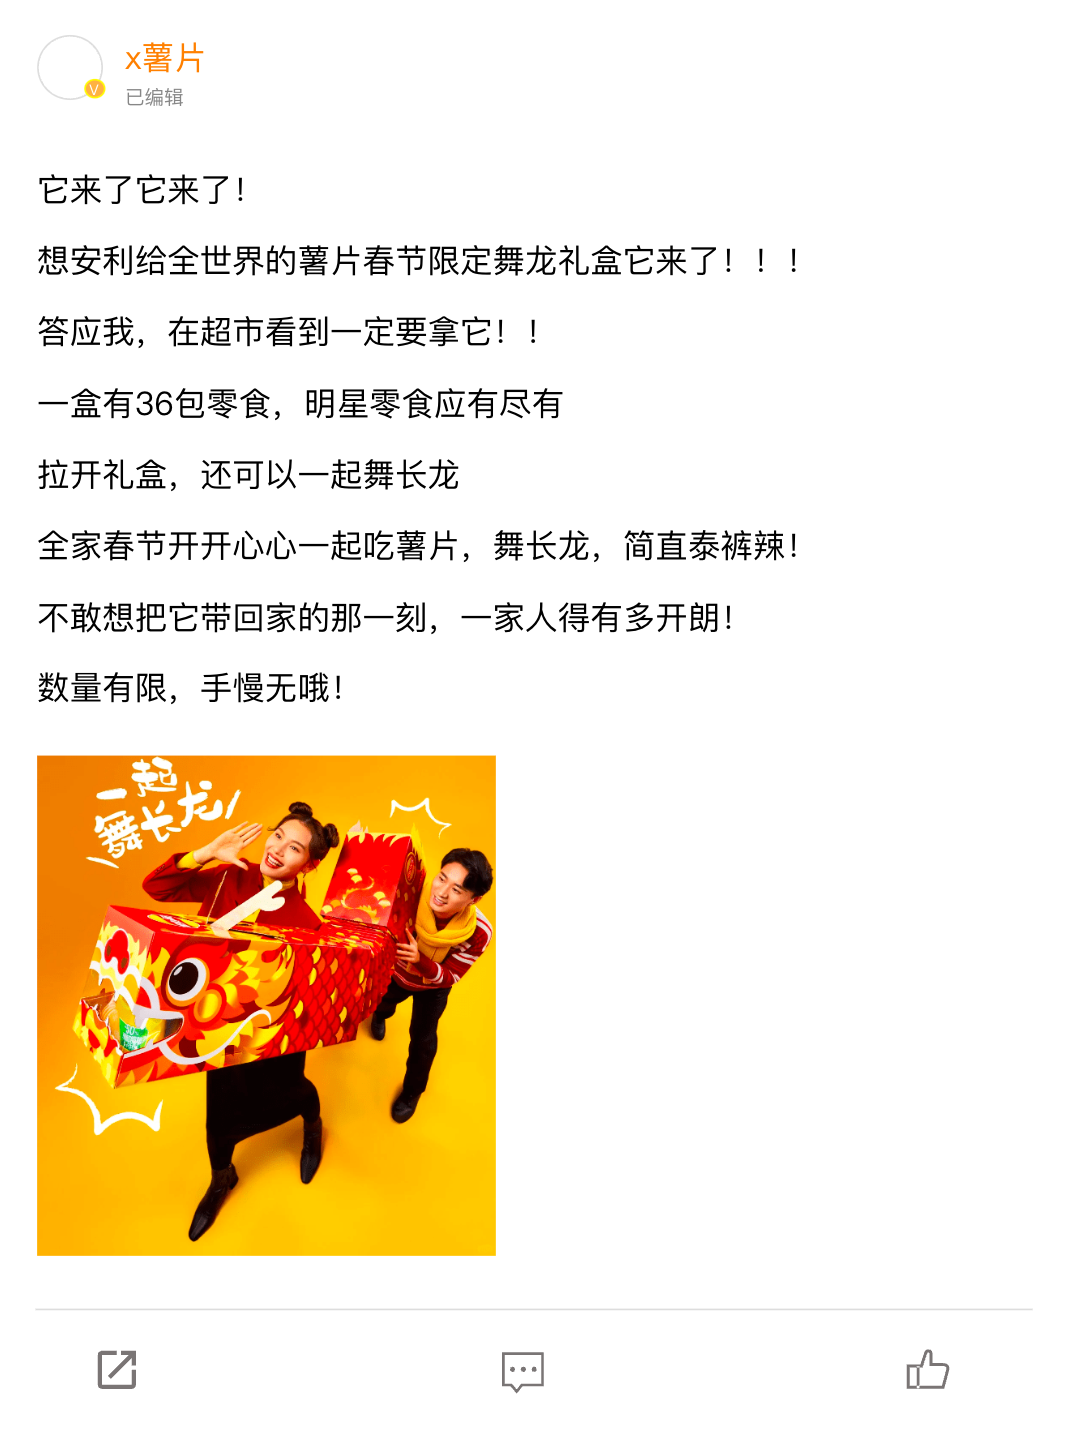
\includegraphics[width=.3\linewidth]{Image/Study1-exp2-ads.png}
    \caption{\label{fig:Study1-exp2-ads}实验开始前的广告示意图}
\end{figure}

为在正式实验前验证个性化广告的有效性,本研究通过见数平台发布预实验,共有60名参与者自愿参加,完成实验后获得1元人民币作为报酬。每名参与者需对2种产品(薯片和电脑)* 3种广告(中性广告和两种个性化广告)进行评价。评分方式与实验1b的预实验一致。参与者需围绕广告的目标消费者特点对广告进行评分,采用1-5点李克特量表,其中1分表示更符合“低水平”描述,5分表示更符合“高水平”描述。例如,对于针对高尽责性设计的广告,参与者需基于以下特征进行评分,从“粗心的、容易分心的、不拘小节的、做事缺少条理的”到“可靠的、有组织的、自律的、注重细节的、有条理”。预实验结果表明(如表\ref{tab:study1-exp2-pretest-results}),生成的个性化广告有效。与中性广告相比,个性化广告在更大程度上符合目标消费者的特点。

\begin{table}[H]
    \centering
    \caption{\label{tab:study1-exp2-pretest-results} 预实验结果:个性化广告与中性广告评分均值}
    {\tablesongti % 整个表格环境应用宋体六号字体
    \renewcommand{\arraystretch}{1} % 调整行距
    \begin{tabular}{l c c c}
        \toprule
        \textbf{产品} & \textbf{目标个性特质} & \textbf{个性化广告(均值)} & \textbf{中性广告(均值)} \\
        \midrule
        薯片 & 尽责性 & 3.82 & 3.47 \\
        薯片 & 开放性 & 3.94 & 3.70 \\
        电脑 & 尽责性 & 4.07 & 3.57 \\
        电脑 & 开放性 & 4.12 & 3.78 \\
        \bottomrule
    \end{tabular}
    }
\end{table}


\textbf{(3)问卷测量}

a. 大五人格量表。因本实验聚焦开放性和尽责性两个维度,我们从\citet{john1991big}编制44道题目的大五人格量表中筛选对应特质的题目。其中,开放性对应10个题项,尽责性对应9个题项。参与者对每个题项的回答均采用1-5点李克特量表,1分表示“完全不符合”,5分表示“完全符合”。

b. 广告说服效果。实验中,每组中性广告和对应的个性化广告以并排形式随机呈现,分别标记为广告A和广告B。参与者需对两则广告的偏好进行评分,评分采用5点双极量表(如图\ref{fig:study1-exp2-rating-example}),分值范围从“更倾向于广告A”到“更倾向于广告B”。为统一结果解读,分数在统计时进行转换,使得分数越高表示越偏好个性化广告,分数越低表示越偏好中性广告。具体的题项与实验1一致(详见 \ref{study1-substudy1-measurement},包含五个题项,用于评估参与者对广告和产品的态度以及购买意图。每个题项均采用1-5点李克特量表评分,广告说服效果的总评分为五个题项得分的平均值。

\begin{figure}[H]
    \centering
    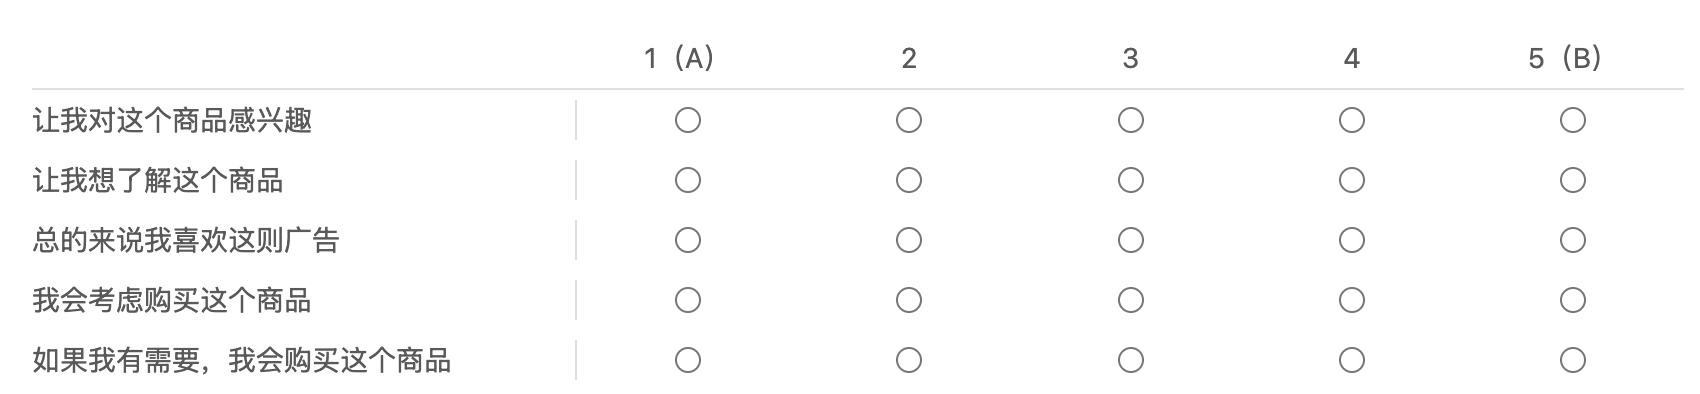
\includegraphics[width=.7\linewidth]{Image/Study1-exp2-rating.png}
    \caption{\label{fig:study1-exp2-rating-example}实验评分示意}
\end{figure}



\subsection{实验流程}
本实验的流程分为两个部分。第一部分,参与者依次阅读每组广告(个性化广告与中性广告并排呈现),并对每组广告的相对说服效果进行评分。广告呈现顺序随机化,以控制顺序效应。第二部分,参与者需回答与人格测试相关的问卷题目,最后提供年龄、性别等人口统计学信息。

\subsection{结果}
我们分别对尽责性个性化广告和开放性个性化广告进行了回归分析。回归模型的自变量包括参与者对应人格特质的得分(尽责性/开放性)、产品类型(电脑/薯片)以及特质与产品类型的交互项,因变量为广告的说服效果。由于评分为二极分布,我们对数据进行了转换,使得得分越高表示相较于中性广告,参与者对个性化广告的偏好越强。

针对尽责性个性化广告,回归模型如下: \begin{equation} Y_{\text{尽责性}} = \beta_0 + \beta_1 \cdot \text{尽责性特质} + \beta_2 \cdot \text{产品类型} + \beta_3 \cdot (\text{尽责性特质} \times \text{产品类型}) + \epsilon \end{equation}

回归分析结果显示,\textbf{尽责性特质的主效应显著}(\textit{$\beta$} = 0.3455, \textit{p} = 0.038),但产品类型的主效应(\textit{$\beta$} = 0.8079, \textit{p} > 0.05)和特质与产品类型的交互项(\textit{$\beta$} = -0.1372, \textit{p} > 0.05)均不显著。这表明,尽责性得分较高的个体相较于中性广告,更偏好针对高尽责性设计的个性化广告,但这种偏好不因产品类型而显著变化。

针对开放性个性化广告,回归模型如下: \begin{equation} Y_{\text{开放性}} = \beta_0 + \beta_1 \cdot \text{开放性特质} + \beta_2 \cdot \text{产品类型} + \beta_3 \cdot (\text{开放性特质} \times \text{产品类型}) + \epsilon \end{equation}

回归分析结果显示,\textbf{开放性特质的主效应显著}(\textit{$\beta$} = 0.3349, \textit{p} = 0.048),但产品类型的主效应(\textit{$\beta$} = -0.9128, \textit{p} > 0.05)和特质与产品类型的交互项(\textit{$\beta$} = 0.1851, \textit{p} > 0.05)均不显著。这表明,开放性得分较高的个体相较于中性广告,更偏好针对高开放性设计的个性化广告,同样,这种偏好不因产品类型的不同而显著变化。
\section{实验3:AI基于中性广告生成高低水平个性化广告的能力}

实验2验证了AI在不同产品类型的中性广告基础上生成个性化广告的能力,结果表明AI能够在享乐型与实用型产品中提取相应的个性化策略,并针对不同人格特质生成有效的个性化广告。然而,实验2仅关注了针对高水平人格特质(如高开放性、高尽责性)的个性化生成,未涉及低水平人格特质的定制设计。在实际应用中,广告不仅需要满足高水平特质个体的需求,还可能需要针对低水平特质个体进行设计,以覆盖更广泛的受众群体。

另一方面,针对高低水平人格特质的个性化效果,在现有文献中并未得到一致的验证。\citet{matz2017psychological}在其大样本实践研究中仅检验了开放性和外倾性分别针对高低水平设计的有效性,未涉及所有人格特质。而在\citet{matz2024potential}基于GPT生成个性化广告的研究中,不同实验间的结果也存在不一致性:部分实验中,针对高低水平设计的个性化广告在开放性、尽责性和外倾性维度上效果显著,但宜人性未能得到稳定的结果。同时,不同因变量(如广告效果与支付意愿)的测量中,高低水平的个性化效果差异也不稳定,尤其是外倾性维度,在某些实验中表现显著,而在另一些实验中则未表现出显著性。

基于上述研究的不一致性,以及实验2未覆盖低水平人格特质的局限,实验3旨在进一步探讨AI在双重人格水平(高水平与低水平)情境下生成个性化广告的能力,并验证高低水平特质的个性化效果是否存在显著差异。这不仅有助于完善现有文献中的空白,也为AI生成的个性化广告在更复杂场景中的应用提供可靠依据。但在本实验中我们不会涉及神经质特质的个性化设计,因为神经质的特性较为独特,其在低水平端的匹配信息(即针对情绪稳定性的设计)往往对高水平和低水平个体均具有吸引力 \citep{matz2016personality},因此难以实现真正针对高低水平的有效区分。


\subsection{方法}


\textbf{(1)被试}

通过见数平台发布实验,356名参与者自愿参加这项研究。36名参与者由于注意检查测试未通过被剔除,剩余\textbf{320名有效参与者}(年龄范围= 18-59岁;\textit{M}=26.06岁;\textit{SD}=7.90;女性200名)。参与任务的每名参与者获得1元人民币作为报酬。注意力检测包含两部分,分别嵌入在因变量测量和人格问卷中,以明确指令题形式呈现(如“请选2”)。参与者需在两道注意力检测题中均作答正确,方可被纳入有效数据样本。每名被试会随机分配到四个特质(开放性、尽责性、外倾性、宜人性)的条件之一,最终每个特质条件均有约80名被试参与。


\textbf{(2)实验材料:广告设计}

本实验共设计\textbf{2(水平:高/低)* 4(特质:开放性、尽责性、外倾性、宜人性)共8则个性化广告}。这些广告均基于一则来自微博平台的热门新款手机中性广告,通过GPT的文本生成与调整功能进行个性化设计。中性广告从当前热门的手机品牌官方广告中筛选而来,考虑到本实验的测量方式旨在比较不同的广告效果,因此品牌效应在比较中被抵消。同时,保留品牌信息能够增强广告的真实性和实验情境的生态效度,因此在本实验中未移除广告中的品牌信息。原广告示例如图\ref{fig:Study1-substudy3-originalAd}所示。针对每个特质与水平的组合,我们使用了GPT生成个性化广告文案(详见附录)。生成过程基于一套结构化的提示语(prompt),提示语(详见附录)包含以下关键要素:任务目标,原始广告文案,调整优化的要求,策略说明。为验证个性化广告的有效性,本研究在正式实验前通过见数平台发布了预实验,共有90名参与者自愿参加,并获得1元人民币作为报酬。每名参与者需对8则广告的目标消费者群体进行选择,具体任务为从2(水平)*5(特质)中选择出最匹配的目标消费者。预实验结果显示,大多数参与者能够正确识别出各广告的目标消费者特质,这表明GPT生成的个性化广告在针对特定人格特质的目标消费者设计上具有有效性。

\begin{figure}[H]
    \centering
    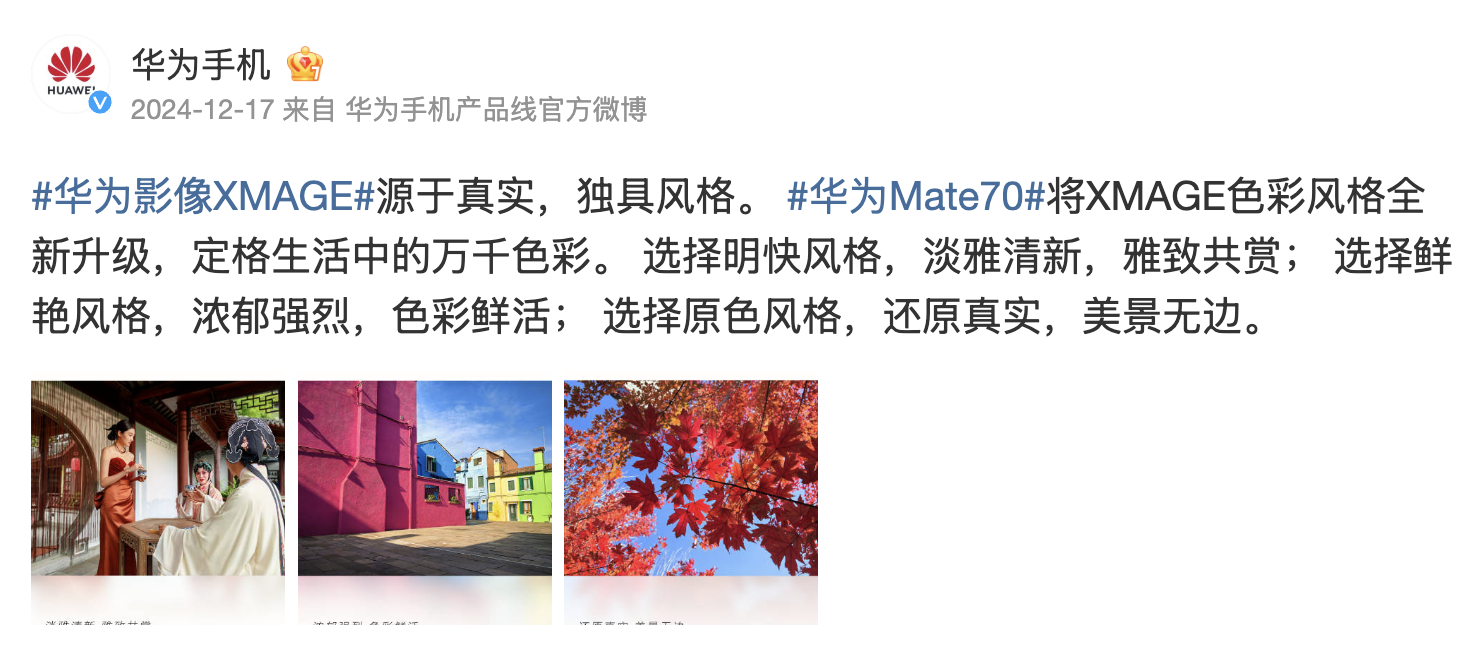
\includegraphics[width=.8\linewidth]{Image/Study1-exp3-original ad.png}
    \caption{\label{fig:Study1-substudy3-originalAd}微博提取广告示意图}
\end{figure}



\textbf{(3)问卷测量}
\label{study1-substudy3-measures}

a. 大五人格量表
本实验从\citet{john1991big}编制的44道题目大五人格量表(BFI-44)中筛选出与目标特质相关的题目。参与者根据其被分配到的人格特质类别完成相应题目。每个题项采用1-5点李克特量表,1分表示“完全不符合”,5分表示“完全符合”。

b. 广告说服效果
实验中,高水平与低水平的个性化广告以并排形式随机呈现,分别标记为广告A和广告B。参与者需对两则广告的偏好进行评分,评分采用11点双极量表(如图\ref{fig:Study1-exp3-rating}),分值范围从“更倾向于广告A”到“更倾向于广告B”。为避免顺序效应,广告A/B呈现顺序随机化。为便于结果解读,在数据统计时将评分结果进行转换,使得分数越高表示参与者对高水平的个性化广告的偏好越强,分数越低表示参与者对低水平的个性化广告的偏好越强。

具体测量题项与实验2保持一致,共包括五个题项,分别评估参与者对广告和产品的态度及其购买意图。广告说服效果的总评分为五个题项得分的平均值。

c. 关键词选择
在广告说服效果评分完成后,参与者还需从每则广告中选出最吸引他们的Top3关键词。这些关键词用于后续分析,以进一步探讨个性化广告的有效性。例如,通过比较高水平与低水平广告中被选出的关键词,评估不同人格特质的参与者是否更倾向于关注与其特质匹配的广告要素。

\begin{figure}[H]
    \centering
    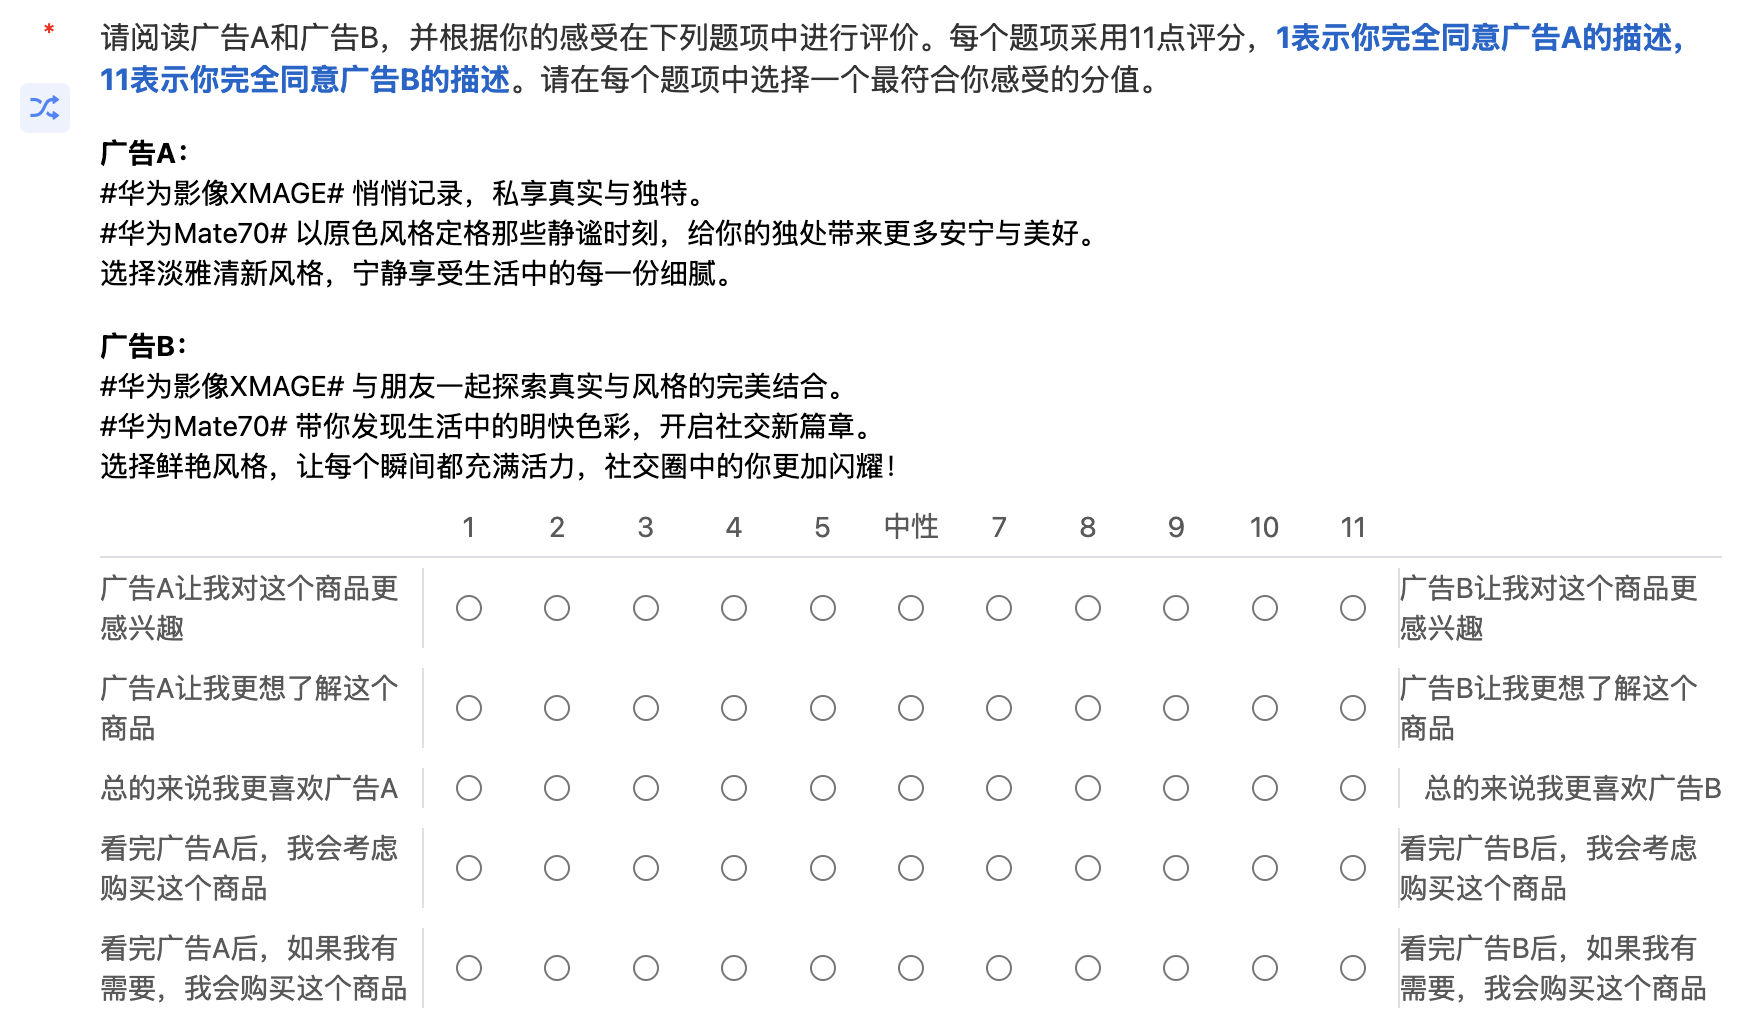
\includegraphics[width=.8\linewidth]{Image/Study1-exp3-rating.png}
    \caption{\label{fig:Study1-exp3-rating}实验评分示意}
\end{figure}


\subsection{实验流程}
本实验流程分为两个部分。第一部分,参与者依次阅读每组广告,其中每组广告包含高水平与低水平的个性化广告(例如,针对高外倾性和低外倾性设计的广告),并对每组广告的相对说服效果进行评分。第二部分,参与者完成与人格测试相关的问卷,随后填写包括年龄、性别等在内的人口统计学信息。

\subsection{结果}
我们分别对每个特质的结果进行了回归分析。回归模型的自变量为参与者对应人格特质的得分(尽责性、开放性、外倾性、宜人性),因变量为广告的说服效果。由于评分为二极分布,我们对数据进行了转换,使得得分越高表示相较于低水平个性化广告,参与者对高水平个性化广告的偏好越强。在这一模型中,如果存在匹配效应(即高水平特质的参与者更偏好针对高水平设计的个性化广告,而低水平特质的参与者更偏好针对低水平设计的个性化广告),则回归系数应为正且显著。

结果如图\ref{fig:Study1-exp3-result}所示,展示了针对四种人格特质设计的广告组的标准化效应及其95\%置信区间。结果表明,开放性(\textit{$\beta$} = 1.729,\textit{p} < 0.01)、外倾性(\textit{$\beta$} = 2.451,\textit{p} < 0.001)和宜人性(\textit{$\beta$} = 1.864,\textit{p} < 0.05)的得分显著预测了参与者对相应特质个性化广告的偏好。这意味着,在这些特质维度上,水平较高的参与者更偏好针对高水平设计的广告,水平较低的参与者则更偏好针对低水平设计的广告。然而,对于尽责性(\textit{$\beta$} = 0.101,\textit{p} = 0.898)维度,未观察到类似的匹配效应,表明无论是高尽责还是低尽责的参与者,在广告偏好上表现出相似的趋势。

\begin{figure}[H]
    \centering
    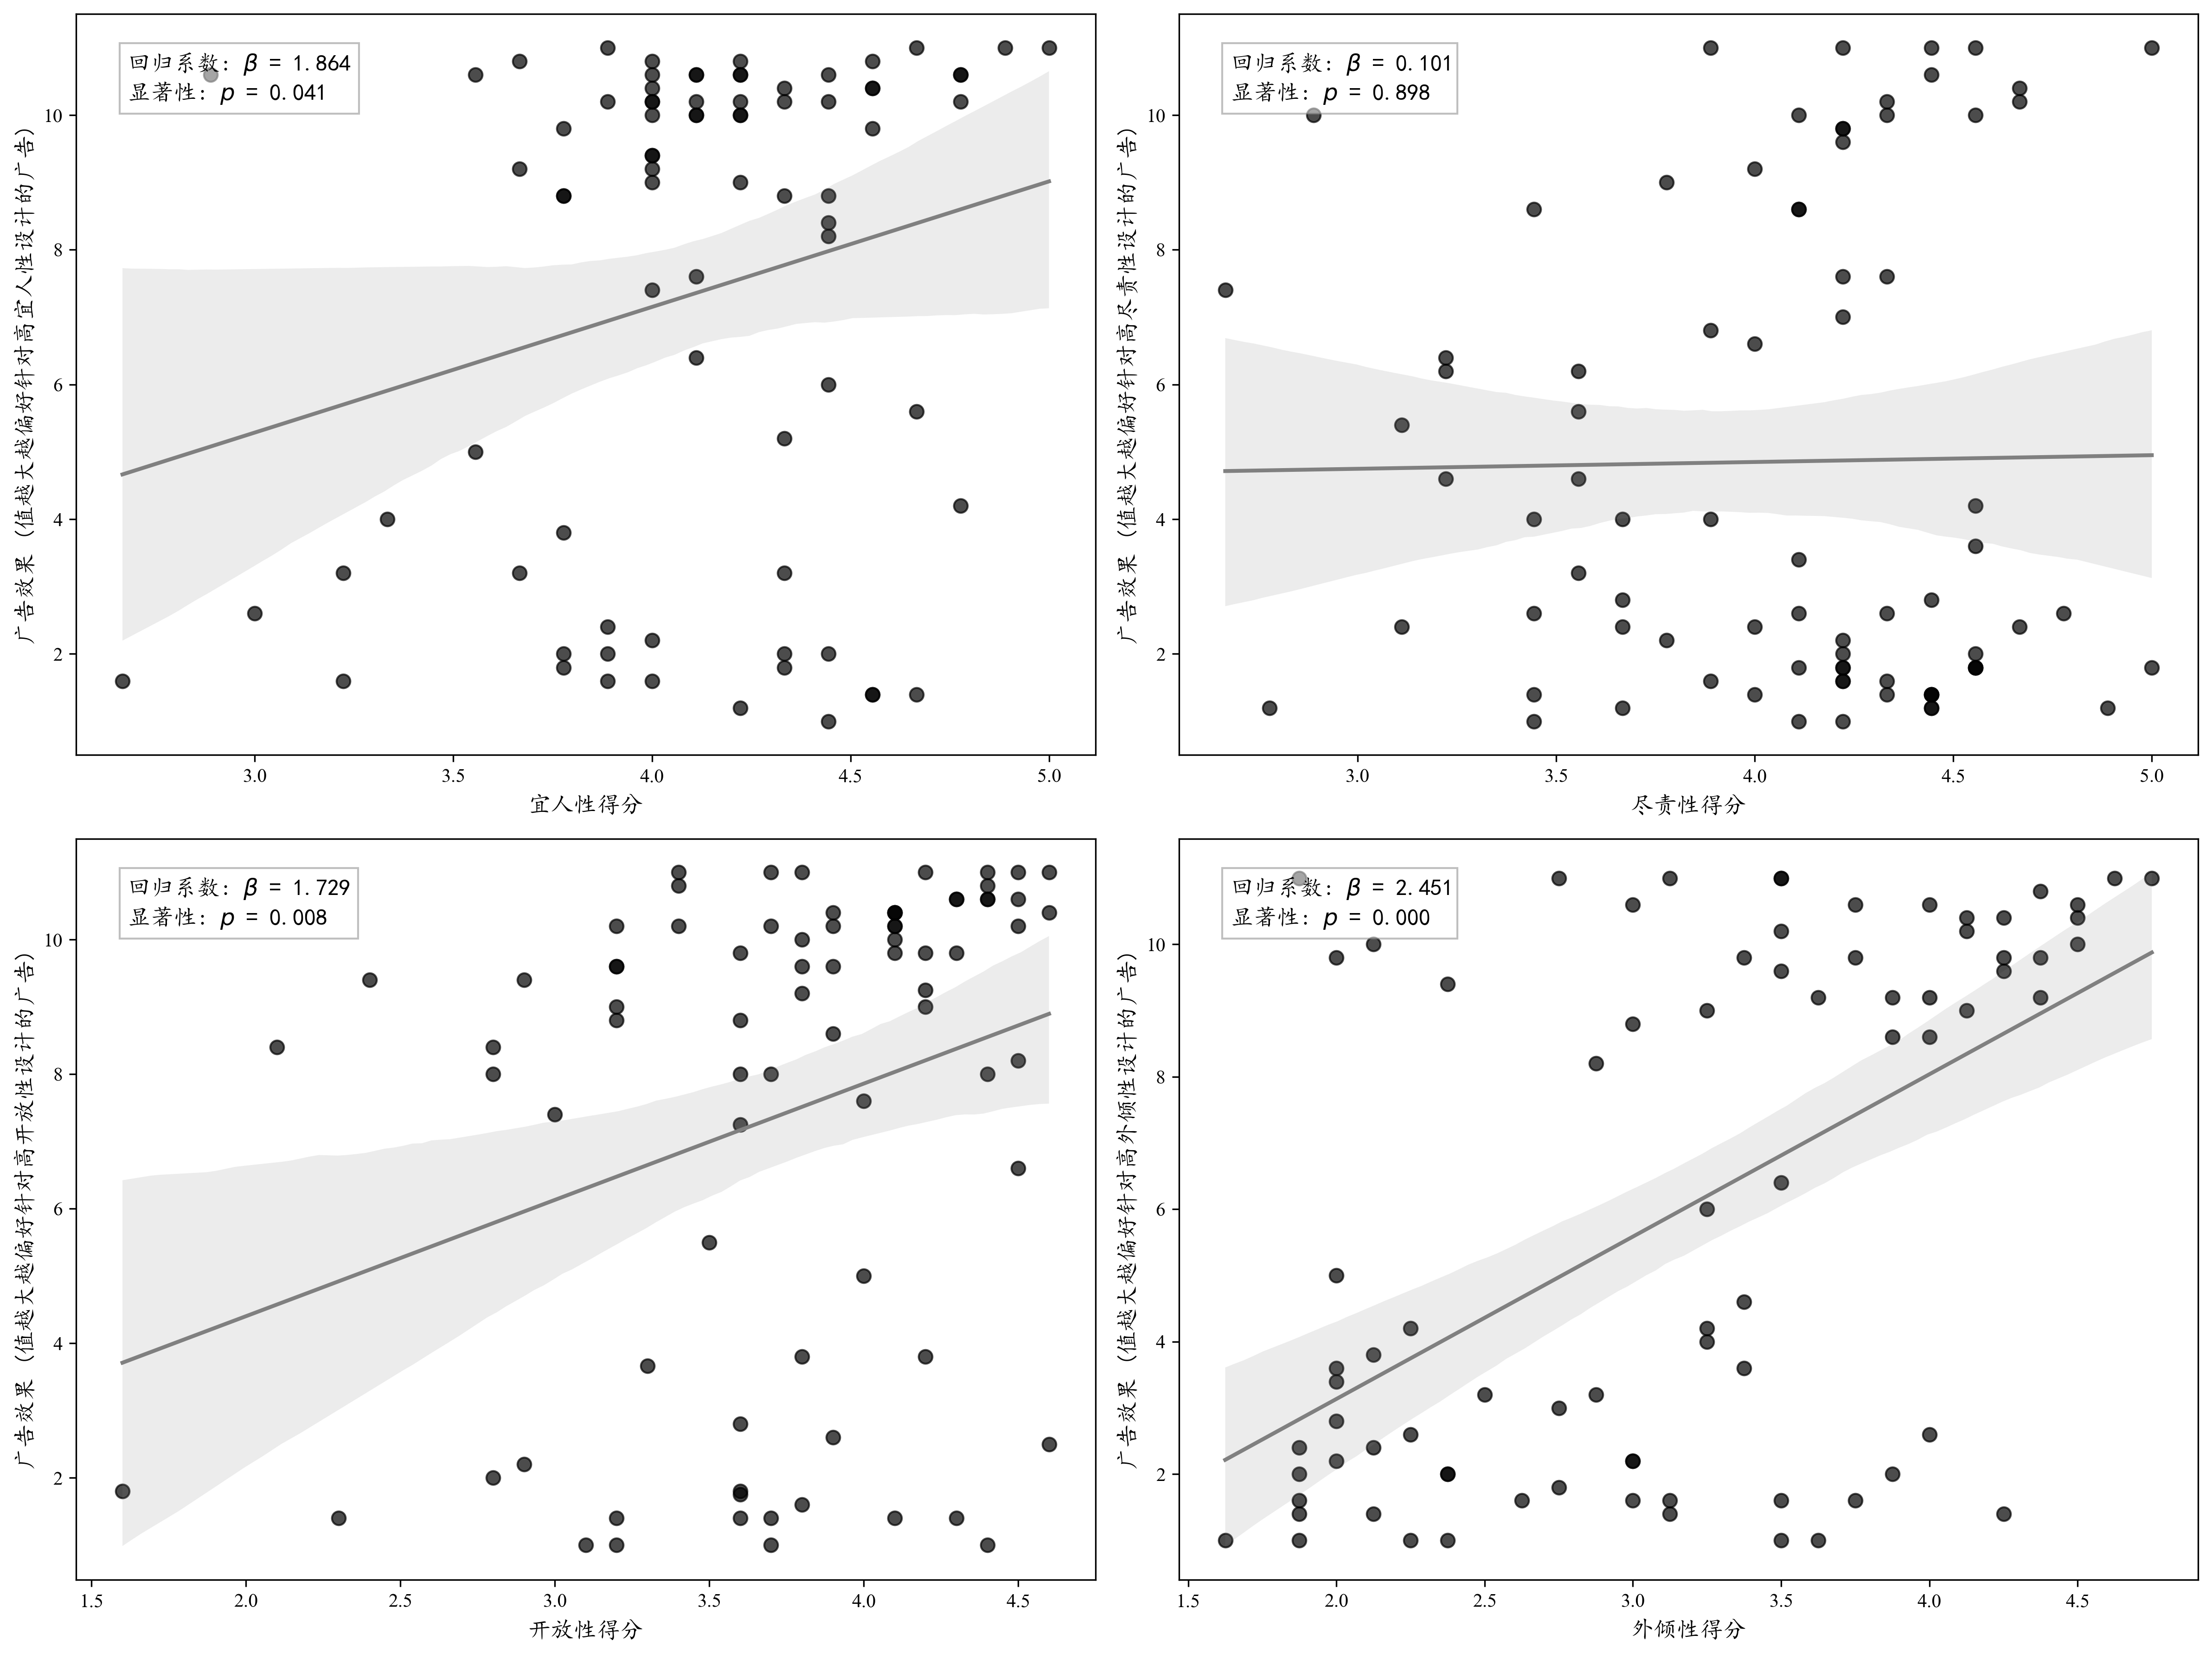
\includegraphics[width=1.0\linewidth]{Image/Study1-exp3-result.png}
    \caption{\label{fig:Study1-exp3-result}四个人格特质对相应广告效果评分的影响(含95\%置信区间)}
\end{figure}

为进一步探讨参与者偏好个性化广告的原因,我们将参与者按人格水平的中值划分为高水平组和低水平组,并筛选出他们在偏好广告中选择的Top 3关键词(根据广告说服效果评分,得分≥6表示更偏好针对高水平设计的广告,<6表示更偏好针对低水平设计的广告),对这些关键词进行词频统计和分析。这种方法能够揭示不同人格水平的个体在广告偏好上的差异,从而帮助解释个性化广告效果的背后机制。

针对回归分析中个性化效果显著的宜人性(表\ref{tab:agreeableness_neutrl_preference})、开放性(表\ref{tab:openness_neutral_preference})和外倾性特质(表\ref{tab:extraversion_neutral_preference}),词频统计结果表明,高水平个体在偏好广告中选择的关键词与广告设计的个性化特征高度一致。例如,在高开放性组中,频繁出现的关键词包括“探索创意”“开启视觉探险”“让想象力成为你的画布”“创新风格”等,这些词语正是针对高开放性设计时所突出的特征,表明个性化广告成功激发了高开放性个体的兴趣和共鸣。然而,对于尽责性特质,尽管回归结果未显示显著的个性化效果,但关键词分析揭示了一些有趣的现象(表\ref{tab:conscientiousness_neutral_preference})。高尽责性组的参与者在偏好广告中也频繁选择了一些针对低尽责性设计的词语,例如“轻松自在”(38.10\%)、“随性而行”(35.71\%)、“享受每一个自由的瞬间”(19.05\%)和“不受拘束”(19.05\%)。虽然这些词语确实也被低尽责性组的参与者广泛选择,但其在高尽责性组中的出现反映出某种交叉偏好。这一现象可能表明,尽责性特质在广告偏好中的表现受到其他特质的影响。例如,高尽责性个体如果同时具有高开放性特质,可能会对这些强调自由和创造性的词语产生共鸣。因此,可以推测当前针对尽责性设计的个性化广告特征还不够突出,导致在高尽责性组中未能显著区分出偏好差异。

综上所述,关键词分析不仅验证了个性化广告在宜人性、开放性和外倾性维度上的有效性,还揭示了尽责性维度个性化效果不显著的可能原因,即现有设计未能充分突出尽责性特质,且其他特质可能对广告偏好产生交互影响。


\definecolor{darkgreen}{RGB}{0,100,0} % 深绿色定义

\begin{table}[htbp]
    \centering
    \caption{\label{tab:agreeableness_neutrl_preference} 高宜人个体与低宜人个体广告词偏好}
    {\tablesongti % 整个表格环境应用宋体六号字体
    \renewcommand{\arraystretch}{1.5} % 调整行距
    \begin{tabularx}{\linewidth}{>{\raggedright\arraybackslash}X c >{\raggedright\arraybackslash}X c}
        \toprule
        \textbf{高宜人个体} & \textbf{比例} & \textbf{低宜人个体} & \textbf{比例} \\
        \midrule
        \textcolor{darkgreen}{捕捉那些充满爱与关怀的温馨瞬间} & \textcolor{darkgreen}{53.33\%} & 捕捉那些充满爱与关怀的温馨瞬间 & 34.29\% \\
        \textcolor{darkgreen}{体贴入微} & \textcolor{darkgreen}{40.00\%} & 体贴入微 & 31.43\% \\
        \textcolor{darkgreen}{让每个微笑都被温柔以待}& \textcolor{darkgreen} {26.67\%} & \textcolor{red}{个性鲜明} & \textcolor{red}{25.71\% }\\
        \textcolor{darkgreen}{你的生活增添和谐美好} & \textcolor{darkgreen} {24.44\%} & \textcolor{red}{独立自主} & \textcolor{red}{22.86\%} \\
        独立自主 & 22.22\% & 让每个微笑都被温柔以待 & 22.86\% \\
        \textcolor{darkgreen}{真诚记录每一次心动} & \textcolor{darkgreen} {20.00\%} & 关怀周到 & 20.00\% \\
        个性鲜明 & 13.33\% & 你的生活增添和谐美好 & 20.00\% \\
        \textcolor{darkgreen}{关怀周到} & \textcolor{darkgreen} {13.33\%} & \textcolor{red}{彰显自我} & \textcolor{red}{17.14\%} \\
        定格每一个独特视角 & 11.11\% & \textcolor{red}{定格每一个独特视角} & \textcolor{red}{17.14\%} \\
        彰显自我 & 6.67\% & 真诚记录每一次心动 & 14.29\% \\
        \bottomrule
    \end{tabularx}
    \vspace{0.1mm}
    \caption*{\raggedright \footnotesize 注:绿色为针对高宜人设计的词语特征,红色为针对低宜人设计的词语特征。}
    }
\end{table}

\begin{table}[htbp]
    \centering
    \caption{\label{tab:openness_neutral_preference} 高开放个体与低开放个体广告词偏好}
    {\tablesongti % 整个表格环境应用宋体六号字体
    \renewcommand{\arraystretch}{1.5} % 调整行距
    \begin{tabularx}{\linewidth}{>{\raggedright\arraybackslash}X c >{\raggedright\arraybackslash}X c}
        \toprule
        \textbf{高开放个体} & \textbf{比例} & \textbf{低开放个体} & \textbf{比例} \\
        \midrule
        \textcolor{darkgreen}{探索创意} & \textcolor{darkgreen}{52.27\%} & \textcolor{red}{经典永恒} & 38.89\% \\
        \textcolor{darkgreen}{开启视觉探险} & \textcolor{darkgreen}{43.18\%} & 探索创意 & 36.11\% \\
        \textcolor{darkgreen}{让想象力成为你的画布} & \textcolor{darkgreen}{38.64\%} & 开启视觉探险 & 33.33\% \\
        \textcolor{darkgreen}{创新风格} & \textcolor{darkgreen}{36.36\%} & 创新风格 & 30.56\% \\
        \textcolor{darkgreen}{无限可能} & \textcolor{darkgreen}{25.00\%} & \textcolor{red}{简单直接} & 30.56\% \\
        \textcolor{darkgreen}{每一次快门都是对未知的好奇} & \textcolor{darkgreen}{22.73\%} & 无限可能 & 22.22\% \\
        经典永恒 & 18.18\% & \textcolor{red}{享受熟悉的舒适} & \textcolor{red}{19.44\%} \\
        简单直接 & 9.09\% & 每一次快门都是对未知的好奇 & 13.89\% \\
        坚持你的风格 & 6.82\% & 让想象力成为你的画布 & 13.89\% \\
        享受熟悉的舒适 & 4.55\% & \textcolor{red}{信赖已知} & \textcolor{red}{13.89\%} \\
        信赖已知 & 2.27\% & \textcolor{red}{坚持你的风格} & \textcolor{red}{5.56\%} \\
        \bottomrule
    \end{tabularx}
    \vspace{0.1mm}
    \caption*{\raggedright \footnotesize 注:绿色为针对高开放设计的词语特征,红色为针对低开放设计的词语特征。}
    
    }
\end{table}

\begin{table}[H]
    \centering
    \caption{\label{tab:extraversion_neutral_preference} 高外倾个体与低外倾个体广告词偏好}
    {\tablesongti % 整个表格环境应用宋体六号字体
    \renewcommand{\arraystretch}{1} % 调整行距
    \begin{tabularx}{\linewidth}{>{\raggedright\arraybackslash}X c >{\raggedright\arraybackslash}X c}
        \toprule
        \textbf{高外倾个体} & \textbf{比例} & \textbf{低外倾个体} & \textbf{比例} \\
        \midrule
        \textcolor{darkgreen}{让每个瞬间都充满活力} & \textcolor{darkgreen}{39.02\%} & \textcolor{red}{私享真实与独特} & \textcolor{red}{46.15\%} \\
        \textcolor{darkgreen}{带你发现生活中的明快色彩} & \textcolor{darkgreen}{31.71\%} & \textcolor{red}{给你的独处带来更多安宁与美好} & \textcolor{red}{41.03\%} \\
        私享真实与独特 & 26.83\% & \textcolor{red}{宁静享受生活中的每一份细腻} & \textcolor{red}{30.77\%} \\
        \textcolor{darkgreen}{开启社交新篇章} & \textcolor{darkgreen}{24.39\%} & \textcolor{red}{定格那些静谧时刻} & \textcolor{red}{28.21\%} \\
        \textcolor{darkgreen}{社交圈中的你更加闪耀} & \textcolor{darkgreen}{24.39\%} & 让每个瞬间都充满活力 & 10.26\% \\
        宁静享受生活中的每一份细腻 & 17.07\% & \textcolor{red}{悄悄记录} & \textcolor{red}{10.26\%} \\
        \textcolor{darkgreen}{与朋友一起探索} & \textcolor{darkgreen}{12.20\%} & 带你发现生活中的明快色彩 & 7.69\% \\
        给你的独处带来更多安宁与美好 & 12.20\% & 社交圈中的你更加闪耀 & 5.13\% \\
        定格那些静谧时刻 & 4.88\% & 与朋友一起探索 & 5.13\% \\
        悄悄记录 & 2.44\% & 开启社交新篇章 & 2.56\% \\
        \bottomrule
    \end{tabularx}
    \vspace{0.1mm}
    \caption*{\raggedright \footnotesize 注:绿色为针对高外倾设计的词语特征,红色为针对低外倾设计的词语特征。}
    }
\end{table}


\begin{table}[H]
    \centering
    \caption{\label{tab:conscientiousness_neutral_preference} 高尽责个体与低尽责个体广告词偏好}
    {\tablesongti % 整个表格环境应用宋体六号字体
    \renewcommand{\arraystretch}{1} % 调整行距
    \begin{tabularx}{\linewidth}{>{\raggedright\arraybackslash}X c >{\raggedright\arraybackslash}X c}
        \toprule
        \textbf{高尽责个体} & \textbf{比例} & \textbf{低尽责个体} & \textbf{比例} \\
        \midrule
        \textcolor{darkgreen}{专业可靠} & \textcolor{darkgreen}{38.10\%} & \textcolor{red}{轻松自在} & \textcolor{red}{36.84\%} \\
        轻松自在 & 38.10\% & \textcolor{red}{享受每一个自由的瞬间} & \textcolor{red}{26.32\%}\\
        让每一天都活泼非凡 & 35.71\% & \textcolor{red}{随心选择色彩} & \textcolor{red}{23.68\%} \\
        随性而行 & 35.71\% & \textcolor{red}{随性而行} & \textcolor{red}{21.05\%} \\
        享受每一个自由的瞬间 & 19.05\% & 专业可靠 & 18.42\% \\
        不受拘束 & 19.05\% & 每个细节都尽善尽美 & 18.42\% \\
        \textcolor{darkgreen}{工作效率} & \textcolor{darkgreen}{14.29\%} & 让每一天都活泼非凡 & 18.42\% \\
        \textcolor{darkgreen}{准确无误} & \textcolor{darkgreen}{11.90\%} & 记录生活 & 15.79\% \\
        \textcolor{darkgreen}{每一个专业细节} & \textcolor{darkgreen}{11.90\%} & 准确无误 & 13.16\% \\
        随心选择色彩 & 7.14\% & 每一个专业细节 & 13.16\% \\
        \textcolor{darkgreen}{每个细节都尽善尽美} & \textcolor{darkgreen}{7.14\%} & \textcolor{red}{不受拘束} & \textcolor{red}{10.53\%} \\
        \textcolor{darkgreen}{精准捕捉} & \textcolor{darkgreen}{7.14\%} & 工作效率 & 10.53\% \\
        \textcolor{darkgreen}{增添工作的效率与精确} & \textcolor{darkgreen}{7.14\%} & 精准捕捉 & 10.53\% \\
        记录生活 & 2.38\% & 增添工作的效率与精确 & 5.26\% \\
        \bottomrule
    \end{tabularx}
    \vspace{0.1mm}
    \caption*{\raggedright \footnotesize 注:绿色为针对高尽责设计的词语特征,红色为针对低尽责设计的词语特征。}
    }
\end{table}


\section{实验4:AI基于产品描述生成高低水平个性化广告的能力}

实验3验证了AI在中性广告基础上,针对高水平和低水平人格特质生成个性化广告的能力,结果显示在开放性、外倾性和宜人性三个维度上,AI能够有效生成符合不同人格特质水平的个性化广告。然而,在尽责性维度上,并未观察到显著的匹配效应,这可能与尽责性特质的内在特性有关,或与现有中性广告的基础信息不足,难以准确区分高低尽责性的偏好有关。

尽管实验3证明了AI在已有中性广告基础上调整生成个性化广告的能力,但实际广告创作中,尤其是针对新品或特定市场推广场景,往往缺乏现成的中性广告作为基础。在这些情境下,品牌通常需要基于产品描述直接创作广告内容。因此,实验4旨在进一步探讨AI是否能够基于产品描述直接生成针对不同人格特质的个性化广告,从而验证其在更复杂应用场景下的个性化生成能力。

此外,相较于实验3基于已有广告的微调生成,实验4的任务要求更高,AI不仅需要理解产品描述的核心信息,还需要准确提取与目标人格特质相关的要素,进而生成符合特定人格偏好的广告内容。因此,实验4的研究将进一步扩展AI生成个性化广告的适用范围,验证其生成高效个性化广告的能力。

\subsection{方法}


\textbf{(1)被试}

通过见数平台发布实验,368名参与者自愿参加这项研究。48名参与者由于注意检查测试未通过被剔除,剩余\textbf{320名有效参与者}(年龄范围= 18-57岁;\textit{M}=25.88岁;\textit{SD}=6.30;女性198名)。参与任务的每名参与者获得1元人民币作为报酬。注意力检测包含两部分,分别嵌入在因变量测量和人格问卷中,以明确指令题形式呈现(如“请选2”)。参与者需在两道注意力检测题中均作答正确,方可被纳入有效数据样本。每名被试会随机分配到四个特质(开放性、尽责性、外倾性、宜人性)的条件之一,最终每个特质条件均有约80名被试参与。


\textbf{(2)实验材料:广告设计}

实验材料生成数量与实验3一致,共设计\textbf{2(水平:高/低)* 4(特质:开放性、尽责性、外倾性、宜人性)共8则个性化广告}。与实验3不同,实验4中的个性化广告不是基于现有的中性广告进行调整,而是直接基于产品描述生成。我们选择了与实验3相同的产品,即华为Mate70,为了确保生成内容的真实性与关联性,我们从百度搜索中找到的第一篇华为Mate70亮点介绍网页中提取了主要产品特性作为输入内容。针对每个特质与水平的组合,我们使用GPT4生成个性化广告文案。生成过程基于一套结构化提示词(详见附录),包含任务目标、产品描述、调整与优化要求、策略说明。具体而言,GPT的任务是根据输入的产品描述,结合高/低水平的目标人格特质,生成针对目标消费者的个性化广告文案(详见附录)。

为验证生成的个性化广告是否能够有效传达针对目标消费者的特质,本研究在正式实验前通过见数平台发布了预实验,共有90名参与者自愿参加,并获得1元人民币作为报酬。每名参与者需阅读8则广告,并从2(水平)* 5(特质描述)中选择出最匹配的目标消费者。预实验结果表明,大多数参与者能够正确识别出广告所针对的人格特质,这表明GPT基于产品描述生成的个性化广告在针对特定人格特质的目标消费者设计上具有有效性。


\textbf{(3)问卷测量}

同实验3(详见\ref{study1-substudy3-measures},分别测量广告说服效果和大五人格量表。


\subsection{实验流程}
本实验流程分为两个部分。第一部分,参与者依次阅读每组广告,其中每组广告包含高水平与低水平的个性化广告(例如,针对高外倾性和低外倾性设计的广告),并对每组广告的相对说服效果进行评分。第二部分,参与者完成与人格测试相关的问卷,随后填写包括年龄、性别等在内的人口统计学信息。

\subsection{结果}
我们分别对每个特质的结果进行了回归分析。回归模型的自变量为参与者对应人格特质的得分(尽责性、开放性、外倾性、宜人性),因变量为广告的说服效果。由于评分为二极分布,我们对数据进行了转换,使得得分越高表示相较于低水平个性化广告,参与者对高水平个性化广告的偏好越强。在这一模型中,如果存在匹配效应(即高水平特质的参与者更偏好针对高水平设计的个性化广告,而低水平特质的参与者更偏好针对低水平设计的个性化广告),则回归系数应为正且显著。

结果如图\ref{fig:Study1-exp3-result}所示,展示了针对四种人格特质设计的广告组的标准化效应及其95\%置信区间。结果显示,仅在开放性(\textit{$\beta$} = 1.896,\textit{p} < 0.01)和外倾性(\textit{$\beta$} = 2.366,\textit{p} < 0.001)维度上观察到显著的个性化效果,即高开放性和高外倾性的个体更偏好针对高水平特质设计的广告,而低开放性和低外倾性的个体则更偏好针对低水平特质设计的广告。在宜人性维度(\textit{$\beta$} = 0.687,\textit{p} = 0.490)上,未发现显著的个性化效果,表明高低宜人性个体在广告偏好上无明显差异。值得注意的是,在尽责性维度上,回归结果呈现出负向的个性化效果(\textit{$\beta$} = -1.721,\textit{p} < 0.05),即高尽责性个体更偏好针对低尽责性设计的广告,而低尽责性个体则更偏好针对高尽责性设计的广告。

\begin{figure}[H]
    \centering
    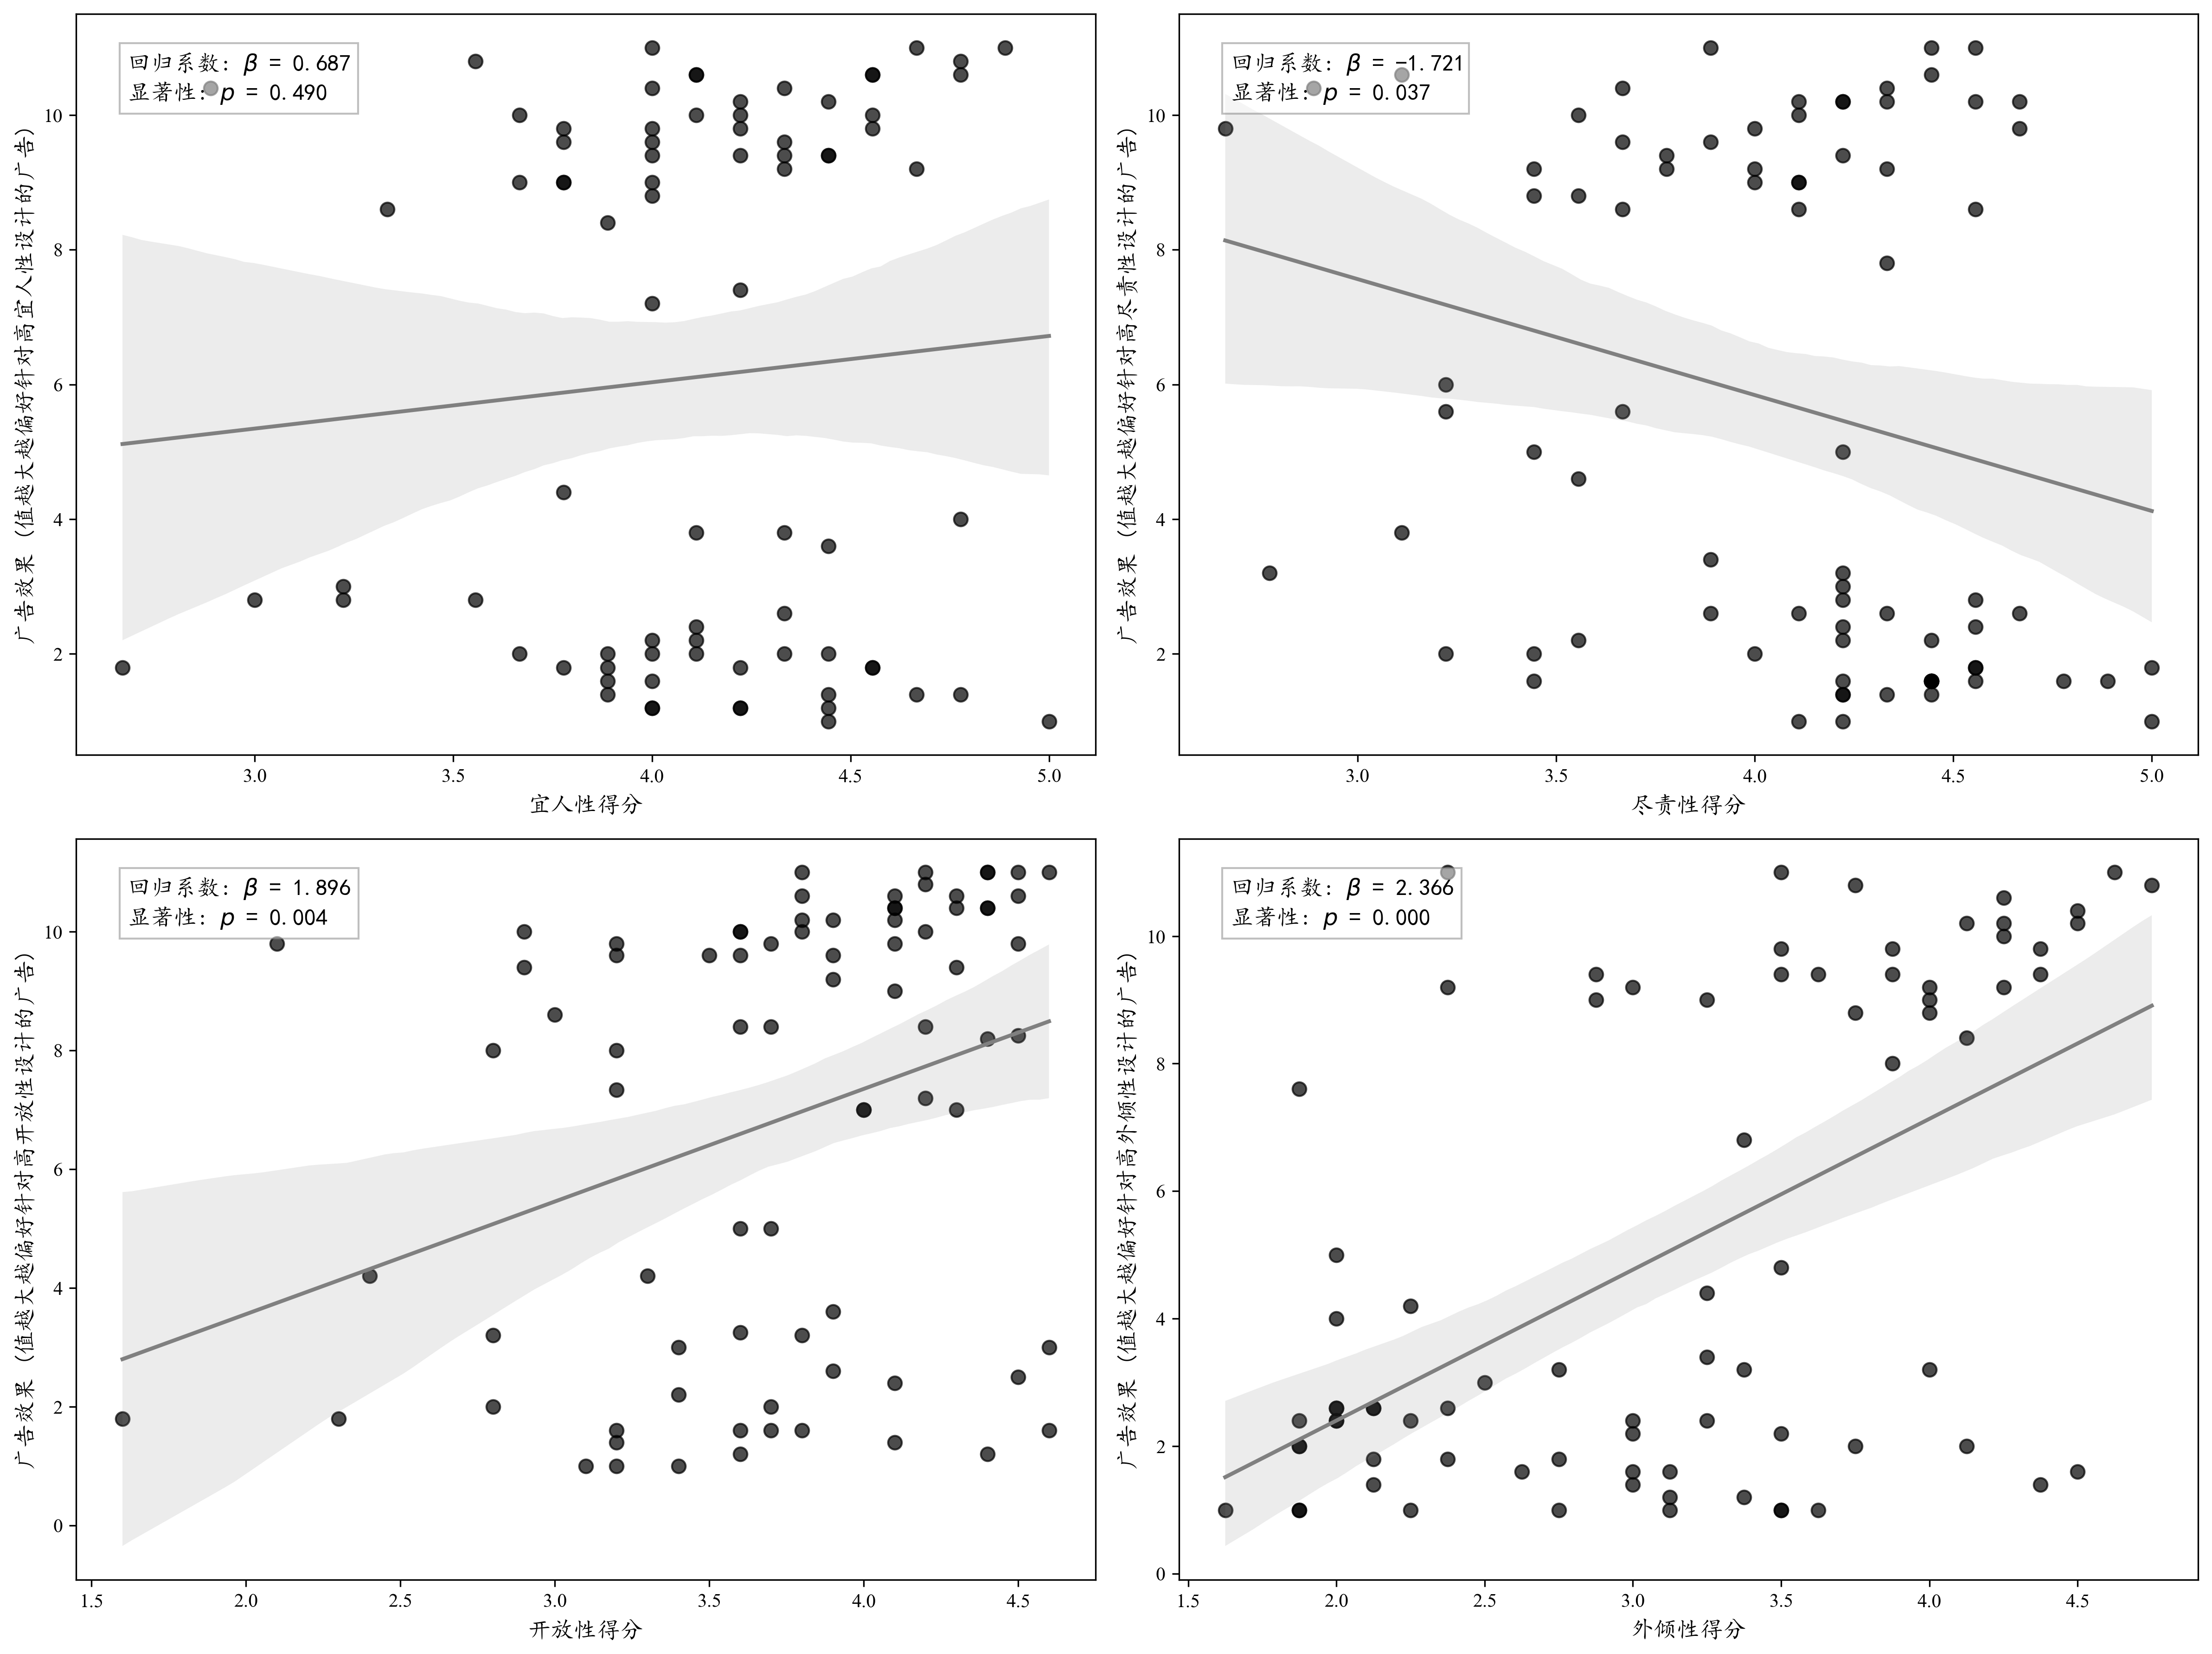
\includegraphics[width=1.0\linewidth]{Image/Study1-exp4-result.png}
    \caption{\label{fig:Study1-exp4-result}四个人格特质对相应广告效果评分的影响(含95\%置信区间)}
\end{figure}

与实验3相同,为进一步探讨参与者偏好个性化广告的原因,我们通过参与者选择的吸引他们的关键词进行分析。对于回归分析中个性化效果显著的开放性和外倾性维度,关键词特征分析结果与个性化设计方向一致。

如表\ref{tab:openness_product_preference}所示,在开放性维度上,高开放性个体偏好的Top关键词包括“无畏创新”(70.45%)、“创意P图”(45.45%)和“探索未知”(43.18%),这些词语正是针对高开放性设计时突出的特征。而低开放性个体偏好的Top关键词为“抗衰耐用”(44.44%)、“简单又可靠”(38.89%)和“创意P图功能”(36.11%),其中前两个词语是针对低开放性设计的特征,而“创意P图功能”则是广告中常见的功能性亮点,因此受到不同类型个体的广泛关注。

如表\ref{tab:extraversion_product_preference}所示,在外倾性维度上,高外倾性个体偏好的Top关键词包括“颜值在线”(36.59\%)、“出场都是焦点”(26.83\%)和“全场瞩目必备”(17.07\%),这些词语明显强调了外倾性个体关注的社交形象和外在表现,与高外倾性个性化设计一致。而低外倾性个体偏好的Top关键词前三位主要为功能性词语,接下来的关键词“无干扰”(23.08\%)、“助力你的个人空间”(23.08\%)和“安静中自由天地”(20.51\%)则与低外倾性特质匹配,突出其对安静和隐私的需求。

对于个性化效果未达到显著水平的宜人性维度(表 \ref{tab:agreeableness_product_preference}),结果呈现出有趣的现象。关键词“充满理解与关怀”(针对高宜人设计,44.44\%)更多被低宜人性个体选择(48.57\%),而“真诚相待”这一针对高宜人设计的词语在低宜人性个体中排名最高(28.57\%)。这表明,在宜人性维度上,个性化设计未能显著区分高低宜人性个体的偏好,可能是由于高低宜人性个体在广告偏好上的差异较小。

对于回归结果呈现负向个性化效果的尽责性维度(表 \ref{tab:conscientiousness_product_preference}),关键词分析结果进一步揭示了这一现象背后的可能原因。一些针对低尽责性设计的关键词,如“简单享受”和“随性而为”,在高尽责性个体中反而被频繁选择,表明这些词语对高尽责性个体也具有吸引力。此外,针对高尽责性设计的关键词,如“100\%信号强度”和“每个细节都完美无瑕”,在低尽责性个体中更受欢迎。这一结果与实验3类似,可能是由于这些词语与开放性特质存在一定的关联性,导致高开放性个体在高尽责性组中对这些词语表现出偏好。

此外,为进一步理解实验中尽责性和宜人性维度未能呈现预期效果的原因,我们参考了先前研究中收集的5110名参与者的人格数据分布(图\ref{fig:Study1-exp4-distribution})。比较发现,本研究中(浅色)宜人性和尽责性维度的分布在高分段聚集了更多被试,这意味着我们的样本中高尽责性和高宜人性个体的比例较高。这一分布特性可能导致偏好上的内部差异性被放大,从而影响了高低水平组的区分效果。例如,在尽责性维度上,高水平组中可能包含了一些具有高开放性特质的个体,而开放性与“简单享受”“随性而为”等词语高度相关,因此这些词语即使针对低尽责性设计,也会被部分高尽责性个体偏好。同样,在宜人性维度上,高水平组内部可能存在更多异质性,导致高宜人性个体未能表现出一致的偏好。因此,数据分布的偏向性可能是导致尽责性和宜人性维度个性化效果未达预期的重要原因。这一结果提示未来研究在划分高低水平组时,应结合更大规模的标准化样本进行比较,或采用连续性指标而非简单的中位数划分,以提高高低水平组的区分精度,进而更准确地检验个性化广告效果。

\begin{table}[H]
    \centering
    \caption{\label{tab:agreeableness_product_preference} 高宜人个体与低宜人个体广告词偏好}
    {\tablesongti % 整个表格环境应用宋体六号字体
    \renewcommand{\arraystretch}{1} % 调整行距
    \begin{tabularx}{\linewidth}{>{\raggedright\arraybackslash}X c >{\raggedright\arraybackslash}X c}
        \toprule
        \textbf{高宜人个体} & \textbf{比例} & \textbf{低宜人个体} & \textbf{比例} \\
        \midrule
        \textcolor{darkgreen}{充满理解与关怀} & \textcolor{darkgreen}{44.44\%} & 充满理解与关怀 & 48.57\% \\
        \textcolor{darkgreen}{用心沟通} & \textcolor{darkgreen}{35.56\%} & \textcolor{red}{AI防窥功能} & \textcolor{red}{31.43\%} \\
        \textcolor{darkgreen}{真诚相待} & \textcolor{darkgreen}{35.56\%} & 真诚相待 & 28.57\% \\
        \textcolor{darkgreen}{不惧真我} & \textcolor{darkgreen}{31.11\%} & \textcolor{red}{保护你的隐私} & \textcolor{red}{28.57\%} \\
        AI防窥功能 & 28.89\% & \textcolor{red}{敢于直言} & \textcolor{red}{25.71\%} \\
        实时AI翻译功能 & 22.22\% & 实时AI翻译功能 & 22.86\% \\
        敢于直言 & 17.78\% & \textcolor{red}{独立自主} & \textcolor{red}{22.86\%} \\
        \textcolor{darkgreen}{保护你的隐私} & \textcolor{darkgreen}{15.56\%} & \textcolor{red}{不惧真我} & \textcolor{red}{20.00\%} \\
        独立自主 & 15.56\% & 用心沟通 & 20.00\% \\
        \textcolor{darkgreen}{温暖科技} & \textcolor{darkgreen}{13.33\%} & 温暖科技 & 11.43\% \\
        \textcolor{darkgreen}{只属于你自己} & \textcolor{darkgreen}{8.89\%} & \textcolor{red}{只属于你自己} & \textcolor{red}{11.43\%} \\
        \bottomrule
    \end{tabularx}
    \vspace{0.1mm}
    \caption*{\raggedright \footnotesize 注:绿色为针对高宜人设计的词语特征,红色为针对低宜人设计的词语特征。}
    }
\end{table}


\begin{table}[H]
    \centering
    \caption{\label{tab:openness_product_preference} 高开放个体与低开放个体广告词偏好}
    {\tablesongti % 整个表格环境应用宋体六号字体
    \renewcommand{\arraystretch}{1} % 调整行距
    \begin{tabularx}{\linewidth}{>{\raggedright\arraybackslash}X c >{\raggedright\arraybackslash}X c}
        \toprule
        \textbf{高开放个体} & \textbf{比例} & \textbf{低开放个体} & \textbf{比例} \\
        \midrule
        \textcolor{darkgreen}{无畏创新} & \textcolor{darkgreen}{70.45\%} & \textcolor{red}{抗摔耐用} & \textcolor{red}{44.44\%} \\
        \textcolor{darkgreen}{创意P图功能} & \textcolor{darkgreen}{45.45\%} & \textcolor{red}{简单又可靠} & \textcolor{red}{38.89\%} \\
        \textcolor{darkgreen}{探索未知} & \textcolor{darkgreen}{43.18\%} & 创意P图功能 & 36.11\% \\
        AI识别 & 22.73\% & AI识别 & 33.33\% \\
        \textcolor{darkgreen}{创意无限} & \textcolor{darkgreen}{20.45\%} & \textcolor{red}{熟悉的经典} & \textcolor{red}{30.56\%} \\
        \textcolor{darkgreen}{激发你的每一个创新想法} & \textcolor{darkgreen}{15.91\%} & 无畏创新 & 27.78\% \\
        \textcolor{darkgreen}{抗摔耐用} & \textcolor{darkgreen}{13.64\%} & \textcolor{red}{让生活更省心} & \textcolor{red}{19.44\%} \\
        简单又可靠 & 13.64\% & 探索未知 & 16.67\% \\
        让生活更省心 & 9.09\% & \textcolor{red}{稳定生活好选择} & \textcolor{red}{11.11\%} \\
        熟悉的经典 & 9.09\% & 轻松应对 & 8.33\% \\
        性能提升 & 6.82\% & 创意无限 & 5.56\% \\
        轻松应对 & 4.55\% & 性能提升 & 5.56\% \\
        & & 每一天的琐碎小事 & 2.78\% \\
        & & 激发你的每一个创新想法 & 2.78\% \\
        \bottomrule
    \end{tabularx}
    \vspace{0.1mm}
    \caption*{\raggedright \footnotesize 注:绿色为针对高开放设计的词语特征,红色为针对低开放设计的词语特征。}
    }
\end{table}

\begin{table}[H]
    \centering
    \caption{\label{tab:extraversion_product_preference} 高外倾个体与低外倾个体广告词偏好}
    {\tablesongti % 整个表格环境应用宋体六号字体
    \renewcommand{\arraystretch}{1} % 调整行距
    \begin{tabularx}{\linewidth}{>{\raggedright\arraybackslash}X c >{\raggedright\arraybackslash}X c}
        \toprule
        \textbf{高外倾个体} & \textbf{比例} & \textbf{低外倾个体} & \textbf{比例} \\
        \midrule
        \textcolor{darkgreen}{颜值在线} & \textcolor{darkgreen}{36.59\%} & AI P图随心创作 & 56.41\% \\
        \textcolor{darkgreen}{出场都是焦点} & \textcolor{darkgreen}{26.83\%} & 零束缚 & 30.77\% \\
        AI P图随心创作 & 26.83\% & 强悍性能 & 28.21\% \\
        无干扰 & 17.07\% & \textcolor{red}{无干扰} & \textcolor{red}{23.08\%} \\
        \textcolor{darkgreen}{全场瞩目必备} & \textcolor{darkgreen}{17.07\%} & \textcolor{red}{助力你的个人空间} & \textcolor{red}{23.08\%} \\
        \textcolor{darkgreen}{让你的社交不再有障碍} & \textcolor{darkgreen}{14.63\%} & 随时捕捉灵感 & 23.08\% \\
        零束缚 & 14.63\% & \textcolor{red}{让你沉浸在属于自己的世界} & \textcolor{red}{20.51\%} \\
        开放式AI翻译 & 12.20\% & \textcolor{red}{安静中自有天地} & \textcolor{red}{20.51\%} \\
        随时捕捉灵感 & 7.32\% & 独处的美好 & 12.82\% \\
        \textcolor{darkgreen}{社交达人首选} & \textcolor{darkgreen}{7.32\%} & 让你的社交不再有障碍 & 7.69\% \\
        强悍性能 & 7.32\% & 开放式AI翻译 & 5.13\% \\
        助力你的个人空间 & 7.32\% & 颜值在线 & 2.56\% \\
        独处的美好 & 4.88\% & 出场都是焦点 & 2.56\% \\
        \textcolor{darkgreen}{让你沉浸在属于自己的世界} & \textcolor{darkgreen}{4.88\%} & 社交达人首选 & 2.56\% \\
        & & 全场瞩目必备 & 2.56\% \\
        \bottomrule
    \end{tabularx}
    \vspace{0.1mm}
    \caption*{\raggedright \footnotesize 注:绿色为针对高外倾设计的词语特征,红色为针对低外倾设计的词语特征。}
    }
\end{table}

\begin{table}[H]
    \centering
    \caption{\label{tab:conscientiousness_product_preference} 高尽责个体与低尽责个体广告词偏好}
    {\tablesongti % 整个表格环境应用宋体六号字体
    \renewcommand{\arraystretch}{1} % 调整行距
    \begin{tabularx}{\linewidth}{>{\raggedright\arraybackslash}X c >{\raggedright\arraybackslash}X c}
        \toprule
        \textbf{高尽责个体} & \textbf{比例} & \textbf{低尽责个体} & \textbf{比例} \\
        \midrule
        简单享受 & 47.62\% & 100\%信号强度 & 44.74\% \\
        便捷的AI功能 & 28.57\% & 每个细节都完美无瑕 & 42.11\% \\
        随性而为 & 26.19\% & 40\%性能提升 & 39.47\% \\
        \textcolor{darkgreen}{100\%信号强度} & \textcolor{darkgreen}{26.19\%} & 为追求卓越而生 & 28.95\% \\
        \textcolor{darkgreen}{每个细节都完美无瑕} & \textcolor{darkgreen}{23.81\%} & 强悍性能 & 26.32\% \\
        \textcolor{darkgreen}{强悍性能} & \textcolor{darkgreen}{21.43\%} & \textcolor{red}{简单享受} & \textcolor{red}{26.32\%} \\
        \textcolor{darkgreen}{40\%性能提升} & \textcolor{darkgreen}{21.43\%} & 便捷的AI功能 & 21.05\% \\
        \textcolor{darkgreen}{为追求卓越而生} & \textcolor{darkgreen}{14.29\%} & \textcolor{red}{随性而为} & \textcolor{red}{15.79\%} \\
        随时随地 & 11.90\% & \textcolor{red}{轻松生活} & \textcolor{red}{15.79\%} \\
        想怎么用就怎么用 & 9.52\% & \textcolor{red}{随时随地} & \textcolor{red}{10.53\%} \\
        轻松生活 & 9.52\% & 专业人士 & 7.89\% \\
        \textcolor{darkgreen}{专业人士} & \textcolor{darkgreen}{4.76\%} & \textcolor{red}{想怎么用就怎么用} & \textcolor{red}{2.63\%} \\
        \bottomrule
    \end{tabularx}
    \vspace{0.1mm}
    \caption*{\raggedright \footnotesize 注:绿色为针对高尽责设计的词语特征,红色为针对低尽责设计的词语特征。}
    }
\end{table}


\begin{figure}[H]
    \centering
    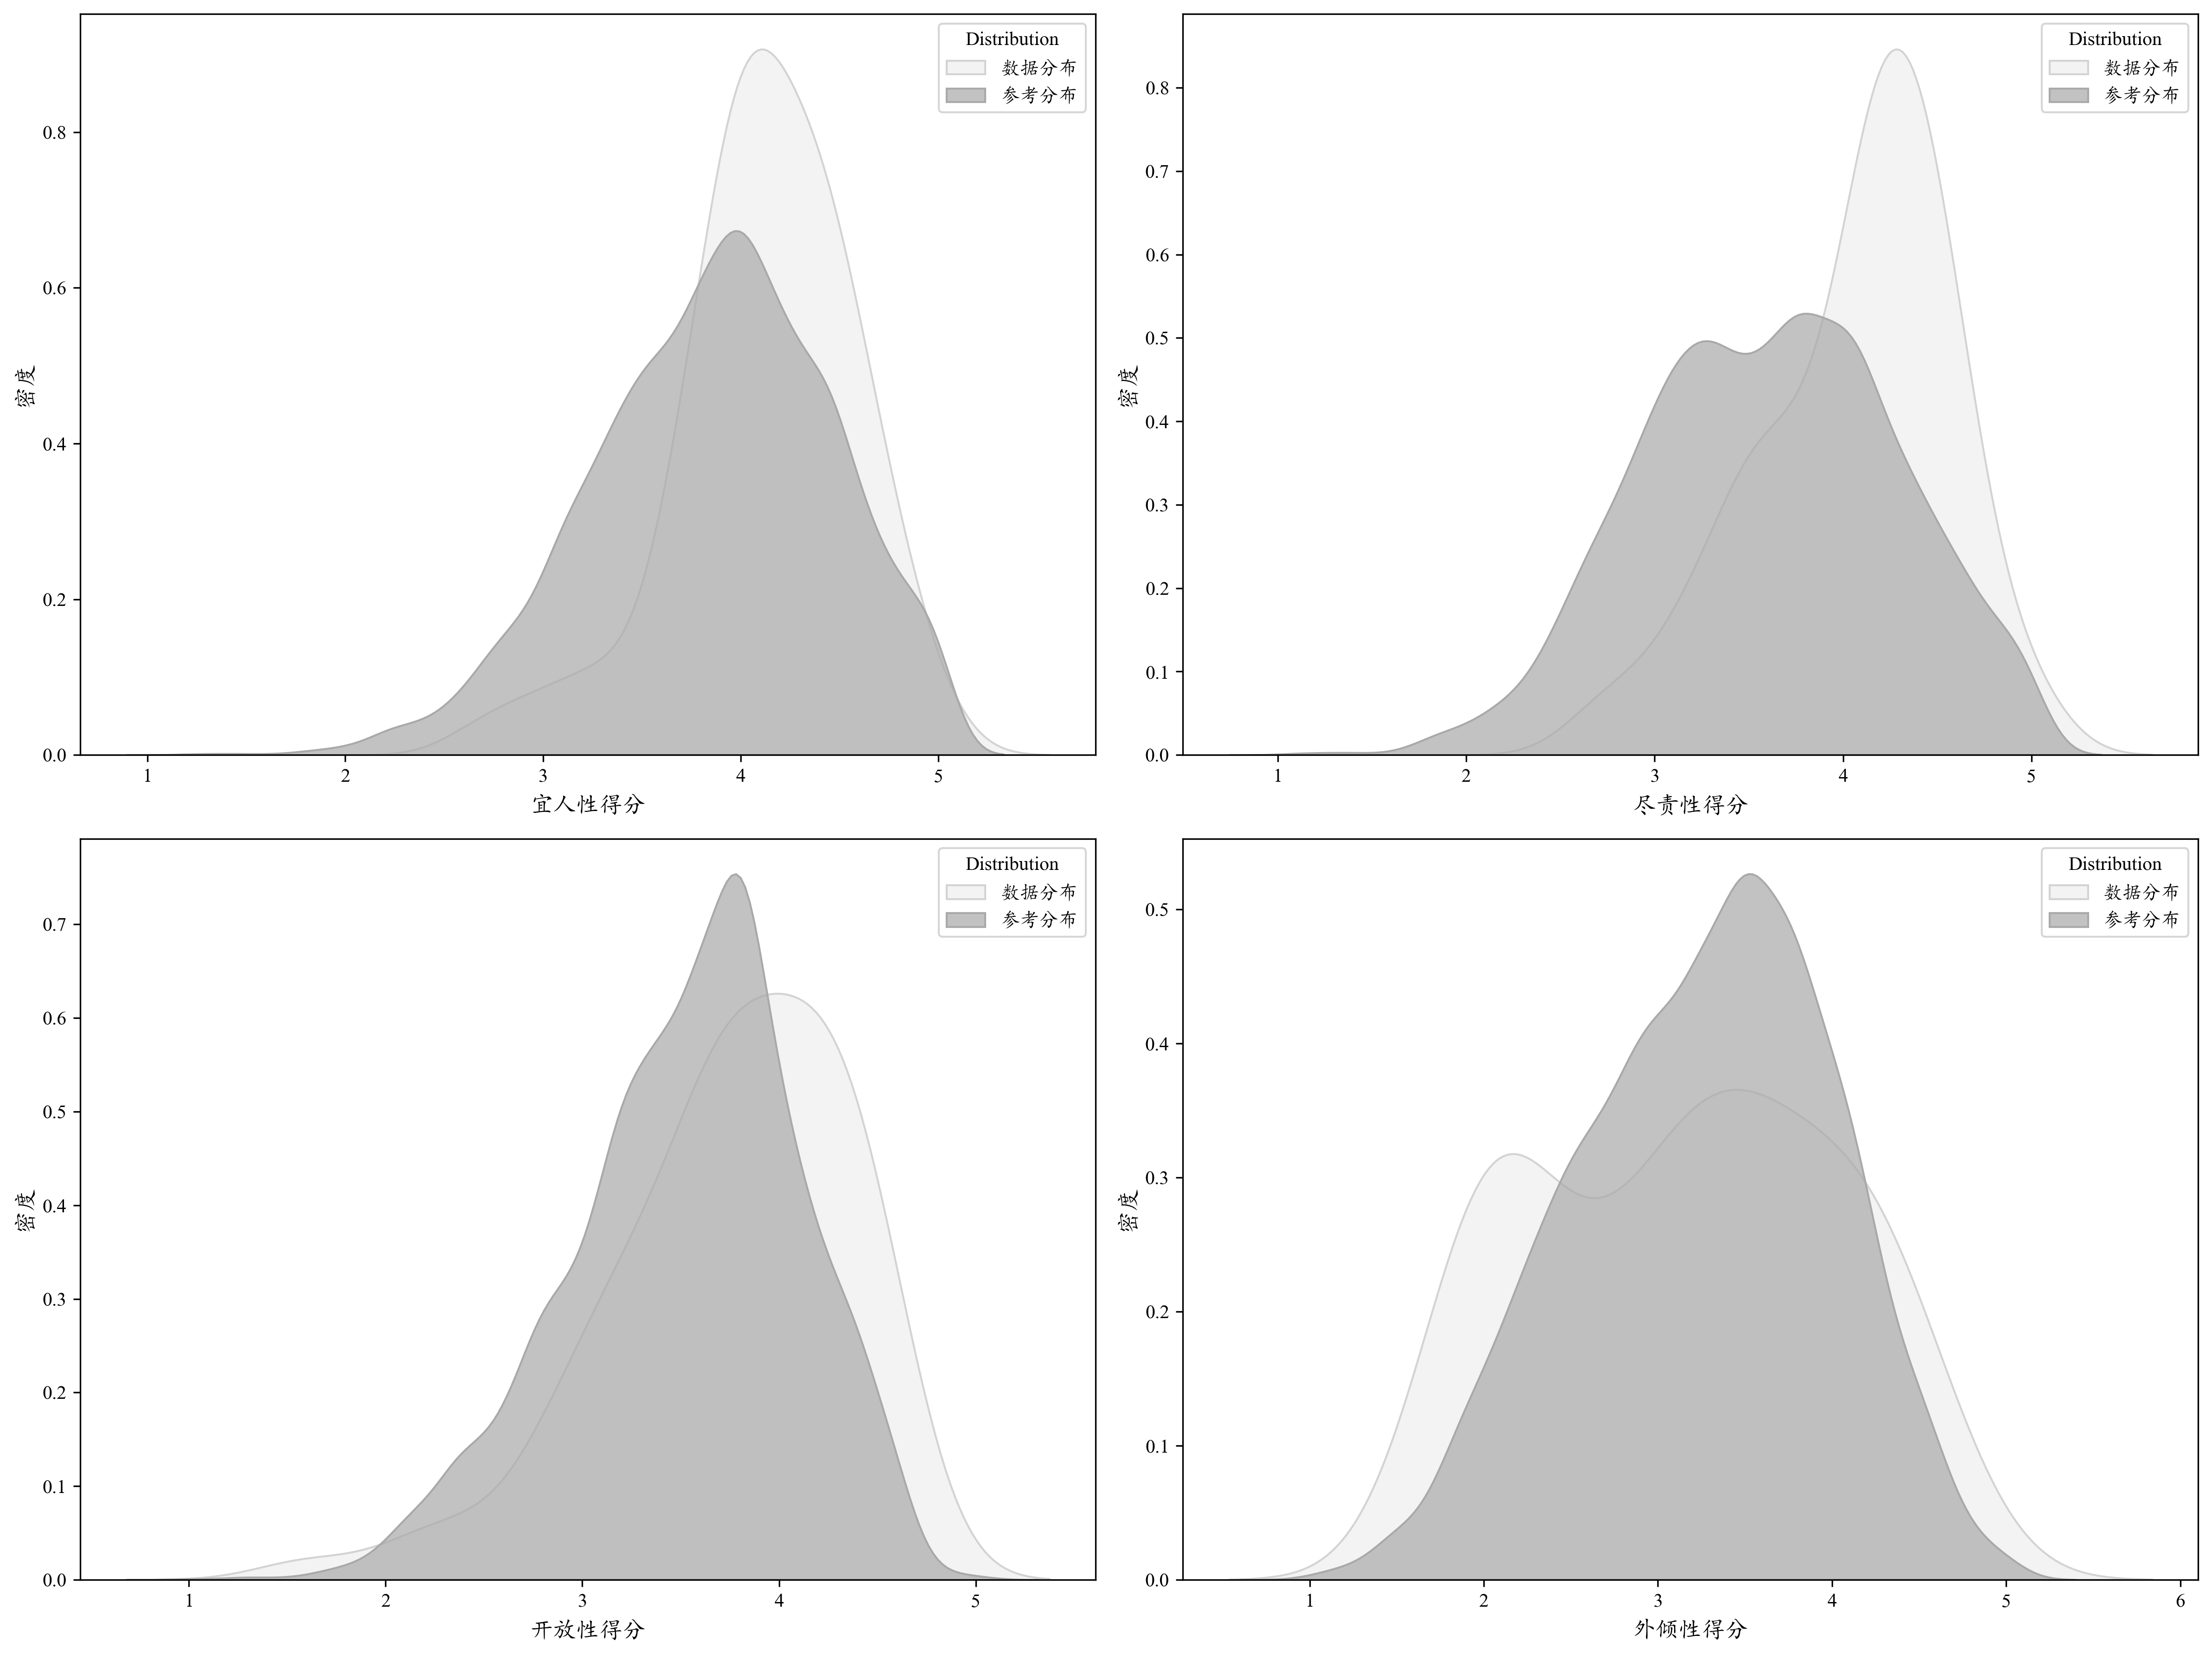
\includegraphics[width=1.0\linewidth]{Image/Study1-exp4-distribution.png}
    \caption{\label{fig:Study1-exp4-distribution}本研究与大样本数据(5110份)的人格特质分布比较}
\end{figure}


\section{讨论}
本研究通过四个实验系统性地探讨了AI基于大五人格特质生成个性化广告的能力,重点关注其在不同人格特质群体中的有效性,并考察了AI在不同广告创作情境下的适用性。研究结果提供了对 AI 生成广告个性化能力的初步验证。

首先\textbf{实验1}作为AI生成个性化广告的初步验证,采用GPT-3.5生成针对大五人格五个维度的个性化广告,结果显示针对\textit{高外倾性}和\textit{高宜人性}设计的个性化广告具有显著的说服效果,\textit{高开放性}呈边缘显著;而\textit{高尽责性}、\textit{高神经质}的广告效果并不显著。这表明AI在某些人格特质群体(如高宜人性和高外倾性)中能够有效生成个性化广告,而在其他人格特质(如高尽责性和高神经质)中,其个性化效果仍存在一定局限。在\textbf{实验2}中,我们进一步考察了AI在不同产品场景下的个性化广告生成能力,并采用GPT-4进行广告创作。实验结果表明,相较于实验1中的 GPT-3.5,GPT-4 能够更有效地生成针对高开放性和高尽责性个体的个性化广告,并在不同产品类型(享乐型 vs. 实用型)中展现出稳定的个性化广告生成能力。这一结果表明,AI 不仅可以基于大五人格进行个性化创作,还能够根据产品类型调整个性化策略,进一步增强广告的针对性和说服力。此外,该实验还验证了AI在基于中性广告进行个性化改写的能力,说明AI可以在已有广告文本的基础上进行个性化调整,而不仅仅是从零生成个性化广告。相较于实验1采用的 GPT-3.5,GPT-4在生成个性化广告方面表现出更强的能力,尤其在开放性和尽责性个体中,其个性化广告的说服力得到了显著提升。这一结果不仅说明 AI 生成的个性化广告效果在不同产品类别中具有一定的稳定性,也表明随着 AI 语言模型能力的提升,其个性化生成效果可能进一步优化。

虽然已有研究表明个性化广告的有效性,但大多数研究仍局限于针对各人格特质的高水平设计 \citep[如][]{hirsh2012personalized,matz2017psychological,winter2021effects}),而对低水平人格特质的个性化广告研究仍然有限,且缺乏系统性探讨。本研究的\textbf{实验3和实验4}进一步考察了AI在不同人格特质水平(高 vs. 低)下的个性化广告生成能力。\textbf{实验3} 结果表明,在\textit{开放性、外倾性和宜人性}维度上,AI生成的个性化广告能够有效匹配目标受众的个性特质,即高水平个体更偏好针对高水平特质设计的广告,低水平个体更偏好针对低水平特质设计的广告。然而,在尽责性维度上,并未观察到显著的匹配效应,这表明尽责性个体的广告偏好可能受其他因素影响,或现有个性化策略仍需进一步优化。此外,关键词分析结果进一步验证了个性化广告的有效性,发现高水平特质个体在广告中更关注符合自身人格特质的关键描述,而低水平特质个体则更倾向于与其匹配的词语特征。在\textbf{实验4}中,我们探讨了AI在基于产品描述直接生成个性化广告的能力,考察其在缺乏中性广告的情况下,是否能够生成符合不同人格特质的个性化广告。结果显示,在\textit{开放性和外倾性}维度上,AI生成的个性化广告仍然表现出显著的匹配效应,高水平特质个体更偏好高水平个性化广告,低水平特质个体则更偏好低水平个性化广告。然而,在\textit{尽责性}维度,个性化效果呈现负向匹配效应,即高尽责性个体更偏好针对低尽责性设计的广告,而低尽责性个体更偏好针对高尽责性设计的广告,这可能与尽责性个体的审慎决策模式有关。此外,在\textit{宜人性维度}上,并未观察到显著的个性化效果,可能是由于宜人性个体的广告偏好差异较小,或是由于实验样本在高宜人性个体中存在较大异质性,影响了个性化匹配的稳定性。这一结果提示,未来研究在优化个性化广告的生成策略时,应进一步考察不同人格特质群体在广告偏好上的具体特征,并结合精细化的提示语(prompt)优化AI生成的广告内容,以提高个性化效果的精准度。

综合来看,本研究对个性化广告的研究进行了补充和拓展。首先,\textbf{实验1和实验2} 说明了AI生成的个性化广告在\textbf{部分人格特质群体}中的有效性,这与\citet{hirsh2012personalized} 和\citet{matz2017psychological} 的结论一致,同时也为\citet{winter2021effects} 提出的个性化广告可能不总是有效的观点提供了新的解释。其次,通过\textbf{实验3和实验4} 的探讨,本研究进一步揭示了\textbf{个性化广告在不同人格水平群体中的匹配效应},并发现尽责性维度的负向匹配效应可能源于广告内容设计与目标群体需求的不匹配。此外,在已有的AI生成个性化广告研究(如\citet{matz2024potential})的基础上,本研究更系统地考察了\textbf{AI在多个生成场景(如基于中性广告改写、基于产品描述直接生成)的个性化能力},并引入了高低人格水平的实验设计,以更全面地检验AI生成个性化广告的有效性。

此外,无论是本研究的研究一,还是既有关于AI在说服性文本生成方面的研究 \citep[如][]{bai2023artificial,goldstein2024persuasive},均主要聚焦于AI本身的能力,而较少涉及AI在与人类专家的直接比较中的表现。然而,以往的说服性研究多基于人类专家或个体创作的文本,因此,将AI与人类专家进行对比不仅能够提供更精确的基准,以衡量AI在个性化广告创作中的实际水平,还能进一步揭示其在不同情境下的适用性与局限性。人类专家长期以来被视为广告创作的标准,其具备更丰富的市场洞察力、更复杂的创意表达方式以及更强的受众情感共鸣能力,而AI则凭借高效的文本生成能力和个性化调整优势,在广告创作中展现出潜在价值。因此,明确AI生成的个性化广告在说服效果上是否能够达到人类专家的水平,或者在人格化定制的特定场景下是否能够展现出特定优势,是一个值得深入探讨的问题。

此外,研究一的结果表明,AI在不同人格特质条件下的个性化广告生成能力并不均衡。例如,在尽责性和宜人性维度上的个性化效果未能稳定显现,甚至在尽责性维度上出现了负向匹配效应。这一现象进一步引发了对于个性化广告稳定性的讨论,即人类专家创作的广告是否能在不同人格特质条件下展现出更稳定的说服效果? 现有文献亦表明,AI的说服效能可能因任务性质和应用情境的不同而存在差异。例如,\citet{huang2023artificial} 研究发现,AI在塑造行为意图方面的效果低于人类专家,但在影响个体感知、态度和实际行为方面,与人类专家并无显著差异。因此,在个性化广告这一特定应用场景下,AI与人类专家在说服力上的比较仍然缺乏系统性的实证研究。AI是否能在广告个性化定制中与专家的创作水平相匹配?不同人格特质群体对于AI与专家创作的广告是否存在差异化的接受度?这些问题将在研究二中展开系统性探讨,以进一步评估AI在个性化广告中的优势与局限,并深化对AI生成广告在实际市场应用中的有效性及边界的理解。